\documentclass[10pt,onecolumn]{book}

\usepackage{times} % font
\usepackage{graphicx} % picture reference
\usepackage{amsmath} % split of mathematical formulas
\usepackage{amssymb} % special mathematical symbols
\usepackage{geometry} % margin
\usepackage{setspace} % letter-spacing
\usepackage{indentfirst} % indent
\geometry{left=2cm,right=2cm, top=2cm, bottom=2cm}
\usepackage{hyperref} % hyperlink
\usepackage{cite}
\usepackage[sectionbib]{chapterbib}

\usepackage{multirow}
%\usepackage{color}
\usepackage{ulem}
%\usepackage{todonotes}
\usepackage{xargs}
\usepackage[pdftex,dvipsnames]{xcolor}
\usepackage[colorinlistoftodos,prependcaption]{todonotes}
\newcommandx{\note}[2][1=]{\todo[linecolor=yellow,backgroundcolor=yellow!25,bordercolor=yellow,#1]{#2}}
\newcommandx{\unsure}[2][1=]{\todo[linecolor=red,backgroundcolor=red!25,bordercolor=red,#1]{#2}}
\newcommandx{\improvement}[2][1=]{\todo[linecolor=Plum,backgroundcolor=Plum!25,bordercolor=Plum,#1]{#2}}

%\numberwithin{equation}{section} % the number of equation

%\usepackage{fancy}%页眉页脚包
%\pagestyle{plain}%页眉页脚设置
\usepackage{fancyhdr}
\pagestyle{fancy}

% code
\usepackage{listings}
\usepackage{xcolor}
\usepackage{tcolorbox}

\usepackage{boxedminipage}
\usepackage{algorithm, algorithmic}

\setcounter{MaxMatrixCols}{20}

\def\ie{\emph{i.e.}}
\def\eg{\emph{e.g.}}
\def\etal{\em {et al.}}

\newcommand{\bm}[1]{\mbox{\boldmath{$#1$}}}
\newcommand{\figref}[1]{Fig. \ref{#1}}
\newcommand{\tabref}[1]{Tab. \ref{#1}}
\newcommand{\equref}[1]{(\ref{#1})}
\newcommand{\secref}[1]{Sect. \ref{#1}}
\newcommand{\algref}[1]{Alg. \ref{#1}}
\newcommand{\myPara}[1]{\vspace{.05in}\noindent\textbf{#1}}
\newcommand{\rev}[1]{\textcolor{blue}{#1}}
\newcommand{\rr}[1]{\textcolor{red}{#1}}
\newcommand{\cg}[1]{\textcolor{green}{#1}}
\newcommand{\bb}[1]{\textcolor{blue}{#1}}
\newcommand{\bl}[1]{\textbf{#1}}
\newcommand{\ul}[1]{\underline{#1}}
\newcommand{\mc}[1]{\mathcal{#1}}
\newcommand{\mb}[1]{\mathbb{#1}}

\begin{document}
\date{}

\title{\textbf{Mathematics, Machine Learning and Deep Learning Notes}}

\author{Jinming Su}
\date{Last update: \today}

\maketitle

\thispagestyle{empty}
\newpage
\pagenumbering{Roman}
\newpage
\tableofcontents
%\newpage
%\listoffigures
%\newpage
%\listoftables
%\newpage
%\pagenumbering{arabic}
\newpage
\listoftodos

\newpage
\pagenumbering{arabic}
\mainmatter

\chapter{Mathematical Foundation}
\section{Advanced math}
\subsection{Taylor formula}
General term formula:
\begin{equation}
f(x) = \frac{f(x_0)}{0!} + \frac{f'(x_0)}{1!}(x - x_0) + \frac{f''(x_0)}{2!}(x - x_0)^2 + \cdots + \frac{f^{(n)}(x_0)}{n!}(x - x_0)^n + R_n(x),
\end{equation}
which is the Taylor expansion of $f(x)$ at $x_0$ and $R_n(x)$ means the remainder of Taylor formula.

There are some common Taylor formulas:
\begin{equation}
\begin{split}
e^x = 1 + \frac{x}{1!} + \frac{x^2}{2!} + \frac{x^3}{3!} + \cdot \cdot \cdot + \cdot \cdot \cdot + \frac{x^n}{n!} + R_n = \sum_{i=0}^{\infty} \frac{x^i}{i!}.
\end{split}
\end{equation}

\section{Probability theory and mathematical statistics}
\textbf{Probability theory} mainly focuses on the probability of occurrence of a single event, while \textbf{mathematical statistics} is more inclined to statistics. It focuses on the sampling probability of a group and the possible interval of occurrence of this probability.

In the following introduction, these two concepts are introducted without distinction. 

\subsection{How to get expected value and variance?}
$X$ is a random variable whose values are $X_{1}, X_{2}, ..., X_{n}$. $P(X_{1}), P(X_{2}), ..., P(X_{n})$ are the probability corresponding to these values. The expected value of $X$ can be denoted as $E(X)$, and the variance is denoted as $Var(X)$. Then, 
\begin{equation}
\begin{split}
	E(X) & = \sum_{i = 1}^{n} X_{i}P(X_{i}) \text{\ for discrete variable} \\
		 & = \int_{X}xf(x)dx \text{\ for continous variable} \\	
\end{split},
\end{equation}
and
\begin{equation}
\begin{split}
	Var(X) & = \sum_{i = 1}^{n} (X_{i} - E(X))^2 P(X_{i}) \text{\ for discrete variable} \\
		 & = \int_{X}(x - E(X))^2 f(x) dx  \text{\ for continous variable} \\	
\end{split}.
\end{equation}
For discrete variable, 
\begin{equation}
\begin{split}
	Var(X) & = \sum_{i = 1}^{n} (X_{i} - E(X))^2 P(X_{i}) \\
		   & = E[(X - E(X))^2] \\
		   & = E[X^2 + E(X)^2 - 2XE(X)] \\
		   & = E(X^2) + E(X)^2 - 2E(X)E(X) \\
		   & = E(X^2) - E(X)^2
\end{split}.
\end{equation}

\subsection{Discrete probability distribution}
\textbf{Bernoulli distribution} is \uline{the discrete probability distribution of a random variable} which takes the value 1 with probability $p$ and the value 0 with probability $q=1-p$. We denote Bernoulli distribution as $B(1, p)$. Mathematically, if $X$ is a random variable with $B(1, p)$, then $P(X=1)=p, P(X=0)=q=1-p$. The probability mass function $f$ of this distribution over possible outcoems k, is 
\begin{equation}
f(k;p) = 
\left\{
	\begin{array}{lr}
	p         & \mathrm{if} \ k = 1,\\
	q = 1 - p & \mathrm{if} \ k = 0. \\
	\end{array}
\right.
\end{equation}
The expected value and invarance  of a Bernoulli variable $X$ are
\begin{equation}\label{eq:bernoulli_distribution_e_var}
\left\{
	\begin{array}{lr}
	E(X) = P(X = 1) \cdot 1 + P(X = 0) \cdot 0 = p, \\
	E(X^2) = P(X = 1) \cdot 1^2 + P(X = 0) \cdot 0^2 = P(X = 1) = p, \\ 
	Var(X) = E(X^2) - E(X)^2 = p - p^2 = p(1 - p) = pq.
	\end{array}
\right.
\end{equation}
\note[inline]{Note in Eq.~\ref{eq:bernoulli_distribution_e_var}, maybe $P(X = 1)$ is equivalent $P(X^2 = 1^2)$, which ensures the establishment of this equation.}

\textbf{Binomial distribution} with parameters $n$ and $p$ is \uline{the discrete probability distribution of the number of successes in a sequence of n independent experiments.} Each experiment is a Bernoulli trial. In general, if the ramdom variable $X$ follows the binomial distribution with parameters $n \in \mathbb{N}$ and $p \in [0, 1]$, we write $X \sim B(n, p)$. The probability of getting exactly $k$ successes in $n$ trails is given by the probability mass function:
\begin{equation}
f(k; n, p) = P(k; n, p) = P(X = k) = \binom{n}{k} p^k (1-p)^{n-k}.
\end{equation}
The expected value and invariance of a Binomial variable $X$ (converted into bernouli distribution for derivation, where $X_{i}$ is independent of each other) are
\begin{equation}\label{eq:binomial_distribution_e_var}
\left\{
	\begin{array}{lr}
	\begin{split}
	E(X)  & = E(X_{1} + X_{2} + \cdot \cdot \cdot X_{n}) \\
		  & = E(X_{1}) + E(X_{2}) + \cdot \cdot \cdot + E(X_{n}) \\
		  & = p + p + \cdot \cdot \cdot + p \\
		  & = np, \\
	\end{split} \\
	\begin{split}
	Var(X) & = Var(X_{1}) + Var(X_{2}) + \cdot \cdot \cdot + Var(X_{n}) \\
		   & = nVar(X_{1}) \\
		   & = np(1-p). \\
	\end{split} 
	\end{array}
\right.
\end{equation}
\note[inline]{There exists another solution directly through derivation of the probability mass function of Binomial distribution.}

\textbf{Poisson distribution} is \uline{a discrete probability distribution that expresses the probability of a given number $k$ of events occurring in a fixed interval of time or space} if these events occure with a known constant rate $\lambda$ and independently of the time since the last events. If $X$ is a Poisson variable with the average number of events $\lambda$, we write $X \sim Possion(\lambda)$. The probability mass function is
\begin{equation}
f(k; n, \lambda) = P(X = k) = \frac{e^{-\lambda} \lambda^k}{k!}.
\end{equation}
The expected value and invariance of a Poission variable $X$ are
\begin{equation}\label{eq:poisson_distribution_e_var}
\left\{
	\begin{array}{lr}
	\begin{split}
	E(X)  & = \sum_{i=0}^{\infty} i P(X = i) \\
		  & = \sum_{i=1}^{\infty} i \frac{e^{-\lambda} \lambda^i}{i!} 
		    = \lambda e^{-\lambda} \sum_{i=1}^{\infty} \frac{\lambda^{i - 1}}{(i - 1)!} 
		    = \lambda e^{-\lambda} \sum_{i=0}^{\infty} \frac{\lambda^{i}}{i!} \\
		  & = \lambda e^{-\lambda} e ^ \lambda \\
		  & = \lambda \\
	\end{split} \\
	\begin{split}
	E(X^2) & = \lambda + \lambda ^ 2 \\
	\end{split} \\
	\begin{split}
	Var(X) & = \lambda + \lambda ^ 2 - \lambda^2 \\
		   & = \lambda \\
	\end{split}  \\
	\end{array}
\right.
\end{equation}
\note[inline]{Note there exists Taylor Expansion (at $x = 0$) $e^x = 1 + \frac{x}{1!} + \frac{x^2}{2!} + \frac{x^3}{3!} + \cdot \cdot \cdot + \cdot \cdot \cdot = \sum_{i=0}^{\infty} \frac{x^i}{i!}$.} 

\subsection{Continuous probability distribution}
For \textbf{continuous uniform distribution}, \uline{all intervals of the same length on the distribution's support are equally probable}. The support is defined by the two parameters, $a$ and $b$, which are its minimum and maximum values. The distribution is often abbreviated $U(a, b)$. The probability density function of the continuous uniform distribution is 
\begin{equation}
f(x)=
\left\{
	\begin{array}{ll}
		\frac{1}{b - a}  & \mathrm{for} \ a \le x \le b,  \\
		0                & \mathrm{for} \ x < a \ \mathrm{or} \ x > b. \\
	\end{array}
\right.
\end{equation}
The expected value and invariance of a Uniform variable $X$ are
\begin{equation}
\left\{
	\begin{array}{lr}
	\begin{split}
	E(X)  & = \int_{a}^{b} x \frac{1}{b - a} \\
		  & = \frac{x^2}{2(b - a)}\bigg|_{a}^b = \frac{b^2 - a^2}{2(b - a)} = \frac{(b + a)(b - a)}{2(b - a)} \\
		  & = \frac{b + a}{2}
	\end{split} \\
	\begin{split}
	E(X^2) & = \int_{a}^{b} x^2 \frac{1}{b - a} \\
		   & = \frac{x^3}{3(b - a)}\bigg|_{a}^b = \frac{b^3 - a^3}{3(b - a)} = \frac{(b - a)(b ^ 2 + a ^ 2 + ab)}{3(b - a)} \\
		   & = \frac{a ^ 2 + b ^ 2 + ab}{3} \\
	\end{split} \\
	\begin{split}
	Var(X) & = E(X^2) - E(X)^2 
		     = \frac{a ^ 2 + b ^ 2 + ab}{3} - (\frac{b + a}{2})^2 \\
		   & = \frac{4a ^ 2 + 4b ^ 2 + 4ab}{12} - \frac{3a^2 + 3b^2 + 6ab}{12} \\
		   & = \frac{(a - b)^2}{12}
	\end{split}  \\
	\end{array}
\right.
\end{equation}

The probability density function of the \textbf{normal distribution} is
\begin{equation}
f(x; \mu, \sigma^2) = \frac{1}{\sqrt{2 \pi \sigma^2}} e^{-\frac{(x - \mu)^2}{2\sigma^2}},
\end{equation}
where $\mu$ is the expectation and $\sigma$ is the standard deviation. If a random variable $X$ is distributed normally with mean $\mu$ and variance $\sigma^2$, one may write $X \sim N(\mu, \sigma^2)$. \note[inline]{The derivation of the expectation and invariance of normal distribution requires multiple integration operations.}

\textbf{Exponential distribution} is the probability distribution that describes the time between events in a Poisson point process, $i.e.$ a process in which event occur continuously and independently at a constant average rate. The distribution is often abbreviated $Exponential(\lambda)$. The probability density function of an exponential distribution is 
\begin{equation}
f(x;\lambda)=
\left\{
	\begin{array}{ll}
		\lambda e ^ {- \lambda x} \ & x \ge 0, \\
		0						    & x < 0.
	\end{array}
\right.
\end{equation}
The expected value and invariance of a Exponential variable $X$ are
\begin{equation}
\left\{
	\begin{array}{lr}
	E(X) = \frac{1}{\lambda}, \\
	Var(X) = \frac{1}{\lambda ^ 2}. \\	
	\end{array}
\right.
\end{equation}
\note[inline]{The derivation of the expectation and invariance of exponential distribution requires multiple integration operations.}
\improvement[inline]{Todo: conjugate distribution and Beta distribution.}

\subsection{Sample mean and sample variance}
\textbf{Sample mean} is defined as
\begin{equation}
\bar{X} = \frac{1}{n} \sum_{i=1}^n X_i.
\end{equation}

\textbf{Sample Variance} is defined as 
\begin{equation}
S^2 = \frac{1}{n - 1} \sum_{i=1}^n(X_i - \bar{X})^2.
\end{equation}

The above definitions follow the theorem: \uline{sample mean is unbiased estimation of population mean and sample variance is unbiased estimation of population variance.} 

\textbf{proof:}
\begin{equation}\label{eq:unbiased_estimation_of_sample_mean_and_variance}
\begin{split}
E[\bar{X}] &= E[\frac{1}{n} \sum_{i=1}^n X_i] \\
			&= \frac{1}{n} \sum_{i=1}^n E[X_i] \\
			&= \frac{1}{n} n E(X) \\
			&= E(X) \\
E[S^2] &= E[\frac{1}{n - 1} \sum_{i=1}^n(X_i - \bar{X})^2] \\
		&= \frac{1}{n-1}E[\sum_{i=1}^n(X_i ^ 2 + \bar{X} ^ 2 - 2 X_i \bar{X})] \\
		&= \frac{1}{n-1}(E[\sum_{i=1}^nX_i ^ 2] + n\bar{X}^2 - 2n\bar{X}^2) \\
		&= \frac{1}{n-1}(nE[X ^ 2] - nE[\bar{X}^2]) \\
		&= \frac{n}{n-1}(Var[X] + E[X]^2 - Var[\bar{X}] - E[\bar{X}]^2) \\
		&= \frac{n}{n-1}(Var[X] - Var[\bar{X}]) \\
		&= \frac{n}{n-1}(Var[X] - \frac{1}{n}Var[X]) \\
		&= Var[X]
\end{split}
\end{equation}

\chapter{Machine Learning}
\section{Linear regression}
\subsection{Unitary linear regression}
The problem can be denoted as:
\begin{equation}
\begin{split}
f_w(x) &= wx + b, \\
L(w) &= \sum_{i = 1}^n (f_w(x^{(i)}) - y^{(i)})^2 = \sum_{i = 1}^n (wx^{(i)} + b - y^{(i)})^2 \\
\frac{\partial L(w)}{\partial w} &= 2\sum_{i=1}^n (wx^{(i)} + b - y^{(i)}) x^{(i)} , \\
\frac{\partial L(w)}{\partial b} &= 2 \sum_{i = 1}^n (wx^{(i)} + b - y^{(i)}).
\end{split}
\end{equation}

The Unitary linear regression has closed-form resolution. Let the partial derivative be 0, we have  
\begin{equation}
\begin{split}
w &= \frac{\sum_{i=1}^n (y^{(i)} - \bar{y}) x^{(i)}}{\sum_{i=1}^n (x^{(i)} - \bar{x}) x^{(i)}}, \\
b &= \bar{y} - w \bar{x}.
\end{split}
\end{equation}

\section{Linear Gression Least mean square (LMS)} 
We define the prediction of formula about $x$:
\begin{equation}
f_{\vec{w}}(\vec{x}) = \vec{w}^\top \vec{x} = \sum_{i = 1}^k w_i x_i.
\end{equation}
We define the loss function:
\begin{equation}
L(\vec{w}) = \frac{1}{2} \sum_{i=1}^n (f_{\vec{w}}(\vec{x}^{(i)}) - y^{(i)})^2.
\end{equation}

We can solve above problem by gradient descent algorithm (GD). \uline{For gradient descent, we usually use one example for one updation.} We use only one training example $(\vec{x}^{(i)}, y^{(i)})$ for simplicity.
\begin{equation}
\begin{split}
\frac{\partial L(\vec{w})}{\partial w_j} & = \frac{1}{2} \cdot 2 (f_{\vec{w}}(\vec{x}^{(i)}) - y^{(i)}) \cdot \frac{\partial \sum_{i = 1}^k w_i x_i}{\partial w_j} \\
	&= (f_{\vec{w}}(\vec{x}^{(i)}) - y^{(i)}) * x^{(i)}_j, \\
w_j &= w_j + \alpha (f_{\vec{w}}(\vec{x}^{(i)}) - y^{(i)}) * x^{(i)}_j.
\end{split}
\end{equation}

Next, we can also solve the problem by the matrix form.
\begin{equation}
\begin{split}
X  & = \left[
 \begin{matrix}
   x^{(1)}_1 & x^{(1)}_2 & \cdots & x^{(1)}_k \\
   x^{(2)}_1 & x^{(2)}_2 & \cdots & x^{(2)}_k \\
   \vdots & \vdots & \ddots & \vdots \\
   x^{(n)}_1 & x^{(n)}_2 & \cdots & x^{(n)}_k \\
  \end{matrix}
  \right],
Y = \left[
	\begin{matrix}
	y^{(1)} \\
	y^{(2)} \\
	\vdots \\
	y^{(n)} \\
	\end{matrix}
	\right] \\
L_{\vec{w}}(\vec{w}) & = \frac{1}{2}(X\vec{w} - \vec{Y})^\top (X\vec{w} - \vec{Y}) \\
			& = X^\top X \vec{w} - X^\top \vec{Y}, 
\end{split}
\end{equation}

For above derivation, we need to know
\begin{equation}
\begin{split}
& \nabla_{A} \text{tr}AB = B^\top, \\
& \nabla_{A} \text{tr}AB A^\top C = CAB + C^\top A B^\top.
\end{split}
\end{equation}

Next, we have 
\begin{equation}
\vec{w} = (X^\top X)^{-1} X^\top \vec{Y}
\end{equation}

\section{Logistic regression (LR)}
\subsection{Form}
\begin{equation}
h_\theta(x) = g(\theta^T x)= \frac{1}{1 + e^{-\theta^T x}}.
\end{equation}
The form of sigmoid function is 
\begin{equation}
g(z) = \frac{1}{1 + e^{-z}}.
\end{equation}
The derivation of sigmoid function is 
\begin{equation}
g'(z) = g(z)(1-g(z)).
\end{equation}

Let us assume that 
\begin{equation}
\begin{split}
& P(y = 1 | x;\theta) = h_\theta(x), \\
& P(y = 0 | x; \theta) = 1 - h_\theta(x).
\end{split}
\end{equation}
Above equation can be written more compactly as
\begin{equation}
\begin{split}
p(y|x;\theta) = (h_\theta(x)) ^y (1- h_\theta(x))^{1 - y}.
\end{split}
\end{equation}

Assuming that the $m$ training examples are generated independently, we can then obtain the likelihood of the parameters $\theta$ as
\begin{equation}
\begin{split}
L(\theta) &= p(\vec{y} | X; \theta) \\
			&= \prod_{i=1}^m p(y^{(i)} | x^{(i)}; \theta)\\
			&= \prod_{i=1}^m (h_\theta(x)) ^{y^{(i)}} (1- h_\theta(x))^{1 - y^{(i)}}.
\end{split}
\end{equation}

Usually, it will be easier to maximize the log likelihood:
\begin{equation}
\begin{split}
l(\theta) &= \log L(\theta) \\ 
		&= \sum_{i=1}^m y^{(i)} \log h(x^{(i)}) + (1 - y^{(i)}) \log (1 - h(x^{(i)})).
\end{split}
\end{equation}

\note[inline]{The is the opposite number of binary cross entropy loss function.}

\note[inline]{It can be proved that the cross entropy function is a convex function. A detailed proof can be found in the blog \url{https://blog.csdn.net/RHONYN/article/details/80342126}. About the proof of convex function, the first-order function relies on the non-negativity of the second derivative and the higher-order function relies on the semi-postive characterization of Hessian Matrix. Therefore, we can get the global minimum value of cross entropy.}

Lets start by working with just one training example $(x, y)$, and take derivatives to derive the stochastic gradient ascent rule:
\begin{equation}
\begin{split}
\frac{\partial l(\theta)}{\partial \theta_j} = (y^{(i)} - h_\theta(x^{(i)})) x^{(i)}_j.
\end{split}
\end{equation}
Above, we get the stochastic gradient ascent rule:
\begin{equation}
\begin{split}
\theta_j := \theta_j + \alpha (y^{(i)} - h_\theta(\overrightarrow{{x^{(i)}}}))x^{(i)}_j
\end{split}
\end{equation}

\section{Naive Bayes}
\subsection{Prior and posterior}
The prior probability is the probability of \uline{a cause inferred from experience}, denoted as $P(\theta)$. The posterior probability is the probability of \uline{the cause estimated from the result}, denoted as $P(\theta|x)$. The posterior probability is defined as 
\begin{equation}\label{eq:posterior}
\begin{split}
P(\theta|x) = \frac{P(x|\theta) P(\theta)}{P(x)}
\end{split}
\end{equation}
where $P(x|\theta)$ represents likelihood of $x$. \uline{In fact, likelihood is the function of parameters. Likelihood is equal to the probability of the result occurring caused by a cause (paramters) based on the cause.} 

\uline{Likelihood is from the viewpoint of the frequency. In the frequency, the parameter is a true value, not a random variable, so the parameter has no distribution and no probability.}

\subsection{Naive Bayesian Classifier (NBC)}
the naive bayesian classifier can be expressed as
\begin{equation}\label{eq:naive_bayesian_classifier}
\begin{split}
y = f(x) & = \text{arg}\max_{c_k} P(Y = c_k | X = x) \\
		& = \text{arg}\max_{c_k} \frac{P(Y = c_k) \prod_j P(X^{(j)} = x^{(j)} | Y = c_k)}{\sum_k P(Y = c_k) \prod_j P(X^{(j)} = x^{(j)} | Y = c_k)},
\end{split}
\end{equation}
where $x^{(j)}$ means the $j$th features in the feature vector $x$. 

Since the denominator is the same any $c_k$, the above equation \ref{eq:naive_bayesian_classifier} can be simplified as 
\begin{equation}
\begin{split}
y = \text{arg}\max_{c_k} P(Y = c_k) \prod_j P(X^{(j)} = x^{(j)} | Y = c_k).
\end{split}
\end{equation}

\subsection{Parameter estimation of NBC by maximum likelihood estimation (MLE)}
The parameter in NBC that needed to estimate is the prior $P(Y = c_k)$ and likelihood $P(X^{(j)} = x^{(j)} | Y = c_k)$.  
MLEs of prior and likelihood are
\begin{equation}
\begin{split}
P(Y = c_k) & = \frac{\sum_{i = 1}^N I(y_i = c_k)}{N} \\
P(X^{(j)} = a^{(j)} | Y = c_k) & = \frac{\sum_{i=1}^N I (x^{(j)}_i = a_{jl}, y_i = c_k)}{\sum_{i = 1}^N I(y_i = c_k)},
\end{split}
\end{equation}
where $x^{(j)}_i$ is the $j$th feature in $i$th sample vector, and $a_{jl}$ means the $l$th value in the set of values of $j$th feature.

The proof is as follows.
Define $\theta_k = P(Y = c_k)$, then we can get the joint probability distribution.
\begin{equation}
\begin{split}
P(y_1, y_2, \cdots, y_n; \theta_k) = \prod_{i=1}^N P(y_i) = \prod_{i=1}^N \theta_k^{N_k},
\end{split}
\end{equation}
then the likelihood function is 
\begin{equation}
\begin{split}
L(\theta^k; y_1, y_2, \cdots, y_n) = P(y_1, y_2, \cdots, y_n; \theta_k).
\end{split}
\end{equation}
Next, the logarithmic operation is applied.
\begin{equation}
\begin{split}
\ln(L(\theta_k)) = \sum_{i = 1}^N N_k \ln \theta_k, \\
s.t., \sum_{k = 1}^K \theta_k = 1
\end{split}
\end{equation}
Using Lagrange Multiplier Method, we get
\begin{equation}
\begin{split}
\ln(L(\theta_k, \lambda)) = \sum_{i = 1}^N N_k \ln \theta_k + \lambda(\sum_{k = 1}^K \theta_k - 1).
\end{split}
\end{equation}
Let the derivative of the above equation be zero, and combine all the equations with $\theta$. We get 
\begin{equation}
\begin{split}
P(Y=c_k) = \frac{N_k}{N} = \frac{\sum_{i = 1}^N I(y_i = c_k)}{N}.
\end{split}
\end{equation}
Moreover, the derivation of likelihood is similar.

\section{Regularization}

The key purpose of machine learning is to minimize errors of problems while regularizing parameters. \uline{Minimizing errors is to let the model fit the training data, while regularizing parameters is to prevent the model from fitting the training data too much.} 

\uline{Regularization is equivalent to introducing a prior (Laplace or Gaussian).}
In general, supervised learning tasks can be regarded as:
\begin{equation}
w* = \arg\min_w \sum_i L(y_i, f(x_i; w)) + \lambda \Omega(w)
\end{equation}

\begin{figure}[h]
\centering
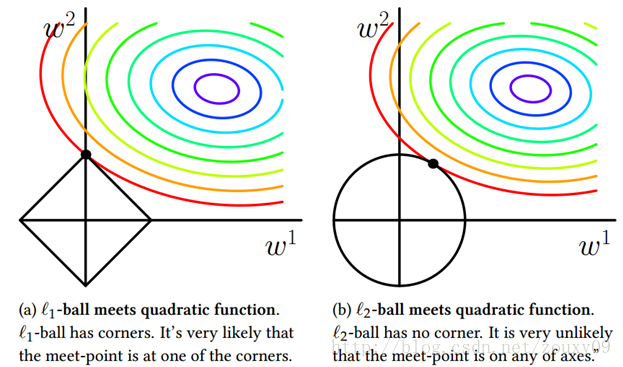
\includegraphics[width=0.4\textwidth]{figures/l1_l2.png}
\caption{$L_1$ norm and $L_2$ norm.}
\end{figure}


\subsection{L0}
\begin{equation}
L_0 = \sum_i \text{I}(w_i \neq 0).
\end{equation}

$L_0$ norm will make the weights sparse.

\subsection{L1 (lasso regularization)}
\begin{equation}
L_1 = \sum_i |w_i|.
\end{equation}

$L_1$ norm will make the weights sparse. The main function of $L_1$ is feature selection and interpretability.

\subsubsection{Why does we usually use L1 to make the weights sparse instead of L0?}

A theoretical explanation is that $L_1$ is the optical convex approximation of $L_0$ while $L_0$ is difficult to solve (NP hard problem). 



\subsection{L2 (ridge regression or weight decay)}
\begin{equation}
L_2 = \sum_i w_i^2
\end{equation}

$L_2$ norm can prevent the model from over-fitting. The main reason is the $L_2$ constrain the model space.

\section{Perceptron}
\subsection{Why can't perceptron solve XOR problem?}
\label{sect:perceptron}
\begin{figure}[h]
\centering
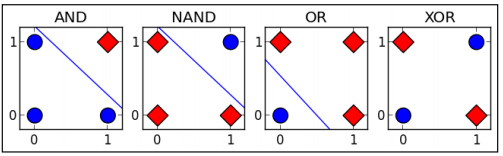
\includegraphics[width=0.4\textwidth]{figures/XOR_problem.png}
\caption{XOR problem.}
\end{figure}
 \uline{Linear classification models can't classify linear non-separable problems.} Perceptron is a linear classificatioin model, and XOR problem is a linear non-separable problem, so perceptron can't solve the XOR problem.

\subsection{Definition of perceptron}
Suppose the input space is $\mathcal{X} \subseteq \mathbb{R}^n$, and the output space is $\mathcal{Y} = \left\{+1, -1\right\}$. For an example $x \in \mathcal{X}$ where $x$ is an n-dimensional vector $(x_{1}, x_{2}, \cdot \cdot \cdot, x_{n})^\mathrm{T}$, $y \in \mathcal{Y}$ represents the category of $x$. Then, we get the perceptron model from the input space to output space: 
\begin{equation}
f(\vec{x}) = \mathrm{sign}(\vec{w}^\mathrm{T} \vec{x} + b),
\end{equation}
where $\vec{w}$ is weight and $b$ is bias. And $\mathrm{sign}$ is a sign function, $i. e.$
\begin{equation}
\mathrm{sign}(x)=
\left\{
	\begin{array}{ll}
		+1, \quad x \ge 0  \\
		-1, \quad x < 0
	\end{array}
\right.
\end{equation}

There exists \uline{a geometric interpretation} that a hyperpalne whose normal vector is $\vec{w}$ and intercept is $b$.

\subsection{Learning Algorithm}
Given a \uline{linear separable} dataset $T = {(x_{1}, y_{1}), (x_{2}, y_{2}), \cdot \cdot \cdot, (x_{N}, y_{N})}$, where $x_{i} \in \mathcal{X} \subseteq \mathbb{R}^n$, and $y_{i} \in \mathcal{Y} = {+1, -1}, i = 1, 2, \cdot \cdot \cdot, N$, we can construct a perspectron model to classify this dataset. 

(1) construct the loss function. we define the loss function as \uline{the total distance from misclassified points to hyperplane}. Toward this end, the distance from any point $x_{0}$ to hyperplane:
\begin{equation}
\frac{1}{||\vec{w}||} |\vec{w}^\mathrm{T}  \cdot \vec{x_{0}} + b|
\end{equation}
where ${||\vec{w}||}$ means the $L_{2}$ norm of $\vec{w}$.\\
\indent As for missclassified points, $\vec{w}^\mathrm{T}  \cdot \vec{x_{0}} + b > 0$ when $y_{i}=-1$, and $\vec{w}^\mathrm{T}  \cdot \vec{x_{0}} + b < 0$ when $y_{i}=+1$. So the total distance from all the misscalssified points to hyperplane is 
\begin{equation}\label{eq:perceptron_loss}
-\frac{1}{||w||}\sum_{\vec{x_{i}} \in M} y_{i} (\vec{w}^\mathrm{T}  \cdot \vec{x_{i}} + b),
\end{equation}
where $M$ is the set of misclassfied points.

\indent \uline{In Eq.~\ref{eq:perceptron_loss}, $\frac{1}{||w||}$ can be ignored. The reason is (a) $\frac{1}{||w||}$ doesn't affcet postive or negative judgment of $y_{i} (\vec{w}^\mathrm{T}  \cdot \vec{x_{i}} + b)$ and (b) $\frac{1}{||w||}$ doesn't affcet the final optimization result of Eq.~\ref{eq:perceptron_loss}. The final optimization result is there are no points with wrong classification, which leads to the loss of 0.} Toward this end, the loss function of preceptron is 
\begin{equation}\label{eq:perceptron_loss}
L(\vec{w}, b) = - \sum_{\vec{x_{i}} \in M} y_{i} (\vec{w}^\mathrm{T}  \cdot \vec{x_{i}} + b),
\end{equation}
and the optimization object is 
\begin{equation}\label{eq:perceptron_loss}
\min_{\vec{w}, b}L(\vec{w}, b) = \min_{\vec{w}, b}- \sum_{\vec{x_{i}} \in M} y_{i} (\vec{w}^\mathrm{T}  \cdot \vec{x_{i}} + b).
\end{equation}

(2) We adopt stochastic gradient descent algorithm to train the perceptron model. Suppose the set of misclassified points is fixed, thus the gradient of loss function $L(\vec{w}, b)$:
\begin{equation}
\begin{split}
	\nabla_{\vec{w}}L(\vec{w}, b) & = - \sum_{\vec{x_i} \in M} y_i \vec{x_i} \\
	\nabla_{b}L(\vec{w}, b)       & = - \sum_{\vec{x_i} \in M} y_i
\end{split}.
\end{equation}
So, the stratagies of $\vec{w}$ and $b$ based on one misclassified point are:
\begin{equation}\label{eq:perceptron_parameter_update}
\begin{split}
	\vec{w} & \gets \vec{w} + \eta y_i \vec{x} \\
	b & \gets b + \eta y_i
\end{split},
\end{equation}
where $\eta$ is the learning rate.

(3) The standard form of perceptron learing algorithm: \\
\indent	\indent input: \uline{linear seperable training set}: $T = \left\{ (x_1, y_1), (x_2, y_2), \cdots, (x_n ,y_n) \right\}$, where $\vec{x_i} \in \mathcal{X} \subseteq \mathbb{R}^n$ and $y_i \in \mathcal{Y} = \left\{-1, +1\right\}, i = 1, 2, \cdots, N$. In addition, the learning rate is denoted 
as $\eta (0 < \eta \le 1)$. \\
\indent \indent output: $\vec{w}, b$. And the perceptron model $f(\vec{x}) = \mathrm{sign}(\vec{w}^\mathrm{T} \vec{x} + b)$. \\
\indent \indent (a) choose initial values, $\vec{w_0}, b_0$, and usually $\vec{w_0} = 0, b_0 = 0$; \\
\indent \indent (b) choose one example $(\vec{x_i}, y_i)$ from the traning set; \\
\indent \indent (c) if $y_{i} (\vec{w}^\mathrm{T}  \cdot \vec{x_{i}} + b) \le 0$:
\begin{equation}
\begin{split}
\vec{w} & \gets \vec{w} + \eta y_i \vec{x} \\
	b & \gets b + \eta y_i
\end{split};
\end{equation} \\
\indent \indent (d)go to (b) until there are no misclassified points in training set.


(4) \note[inline]{The convergence of this algorithm about perceptron leraning can be proved, but it is not within the scope of this note at present.}

\subsection{Dual form of perceptron learning algorithm}
From Eq.~\ref{eq:perceptron_parameter_update}, $\vec{w}$ and $b$ are updated for many times. Suppose the number of updates about each example is $n_i (i = 1, 2, \dots N)$, and we define $\alpha_i = n_i \eta$. Then, the final learned $\vec{w}$ and $b$ can be expressed as
\begin{equation}
\begin{split}
	\vec{w} & = \sum_{i = 1}^{N} \alpha_i y_i \vec{x_i} \\
	b 		& = \sum_{i = 1}^{N} \alpha_i y_i
\end{split}.
\end{equation}

Then, we can obtain the dual form of perceptron learning algorithm.\\
\indent	\indent input: \uline{linear seperable training set}: $T = \left\{ (x_1, y_1), (x_2, y_2), \cdots, (x_n ,y_n) \right\}$, where $\vec{x_i} \in \mathcal{X} \subseteq \mathbb{R}^n$ and $y_i \in \mathcal{Y} = \left\{-1, +1\right\}, i = 1, 2, \cdots, N$. In addition, the learning rate is denoted 
as $\eta (0 < \eta \le 1)$. \\
\indent \indent output: $\vec{\alpha} = (\alpha_1, \alpha_2, \cdots, \alpha_N)^\mathrm{T}, b$. And the perceptron model $f(\vec{x}) = \mathrm{sign}(\sum_{j=1}^{N} \alpha_j y_j \vec{x_j}^\mathrm{T} \vec{x} + b )$. \\
\indent \indent (a) choose initial values, $\vec{\alpha}, b_0$, and usually $\vec{\alpha} = 0, b_0 = 0$; \\
\indent \indent (b) choose one example $(\vec{x_i}, y_i)$ from the traning set; \\
\indent \indent (c) if $y_{i} (\sum_{j=1}^{N} \alpha_j y_j \vec{x_j}^\mathrm{T} \vec{x} + b) \le 0$:
\begin{equation}
\begin{split}
\vec{\alpha_i} & \gets \alpha_i + \eta \\
	b & \gets b + \eta y_i
\end{split};
\end{equation} \\
\indent \indent (d)go to (b) until there are no misclassified points in training set.

\section{Support vector machine (SVM)}
\begin{figure}[h]
\centering
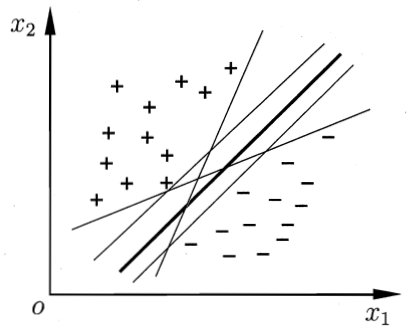
\includegraphics[width=0.3\textwidth]{figures/svm.png}
\caption{Classification hyperplane.}
\end{figure}
\subsection{Form}
For the classification problem, the mathemathcal form of hyperplane is defined as 
\begin{equation}
\begin{split}
\vec{w}^\top \vec{x} + b = 0.
\end{split}
\end{equation}
The distance from any point in the space to the hyperplane is
\begin{equation}
\begin{split}
\gamma = \frac{|\vec{w}^\top \vec{x} + b|}{|\vec{w}|}.
\end{split}
\end{equation}
We know that the class of each points is $y^{(i)}$, where $y^{(i)} = \pm 1$ means different classes. Then, the distance can be in another way by 
\begin{equation}
\begin{split}
\gamma^{(i)} = \frac{y^{(i)}(\vec{w}^\top \overrightarrow{x^{(i)}} + b)}{|\vec{w}|},
\end{split}
\end{equation}
which is named \uline{geometric margin}. Next, we have 
\begin{equation}
\begin{split}
\gamma = \min_{i=1,\cdots, m} \gamma^{(i)}.
\end{split}
\end{equation}

Then, we give the form of SVM as
\begin{equation}\label{eq:svm1}
\begin{split}
& \max_{\gamma, \vec{w}, b} \gamma, \\
& \text{s.t. } \frac{y^{(i)}(\vec{w}^\top \overrightarrow{x^{(i)}} + b)}{|\vec{w}|} \geq \gamma
\end{split}
\end{equation}

Define functional margin as follows.
\begin{equation}
\begin{split}
& \hat{\gamma}^{(i)} = y^{(i)}(\vec{w}^\top \overrightarrow{x^{(i)}} + b), \\
& \hat{\gamma} = \min_{i = 1, \cdots, m} \hat{\gamma}.
\end{split}
\end{equation}

Then, the form of SVM \ref{eq:svm1} can be transformed.
\begin{equation}
\begin{split}
& \max_{\gamma, \vec{w}, b} \frac{\hat{\gamma}}{|\vec{w}|}, \\
& \text{s.t. } y^{(i)}(\vec{w}^\top \overrightarrow{x^{(i)}} + b) \geq \hat{\gamma}.
\end{split}
\end{equation}
We set the minmum functional margin is $\hat{\gamma} = 1$, then 
\begin{equation}\label{eq:svm2}
\begin{split}
& \max_{\gamma, \vec{w}, b} \frac{1}{|\vec{w}|}, \\
& \text{s.t. } y^{(i)}(\vec{w}^\top \overrightarrow{x^{(i)}} + b) \geq 1.
\end{split}
\end{equation}
Moreovere, the form of SVM \ref{eq:svm2} can be transformed.
\begin{equation}\label{eq:svm3}
\begin{split}
& \min_{\gamma, \vec{w}, b} \frac{1}{2}|\vec{w}|^2, \\
& \text{s.t. } y^{(i)}(\vec{w}^\top \overrightarrow{x^{(i)}} + b) \geq 1.
\end{split}
\end{equation}

\subsection{Lagrange duality}
Consider a constrained optimization problems:
\begin{equation}
\begin{split}
\min_w & f(\vec{w}), \\
\text{s.t. } & g_i(\vec{w}) \leq 0, i =1,\cdots, k, \\
			 & h_i(\vec{w}) = 0, i =1, \cdots, l.
\end{split}
\end{equation}
We can define \uline{generalized lagrangian}
\begin{equation}
\mathcal{L}(\vec{w}, \vec{\alpha}, \vec{\beta}) = f(\vec{w}) + \sum_{i = 1}^k \alpha_i g_i(\vec{w}) + \sum_{i = 1}^l \beta_i h_i(\vec{w}).
\end{equation}
If the primal constraints are indeed satisfied for $\vec{w}$, then \uline{$\max_{\vec{\alpha}, \vec{\beta}: \alpha_i \geq 0} \mathcal{L}(\vec{w}, \vec{\alpha}, \vec{\beta}) = f(\vec{w})$ }.

For primal ($p$) and dual ($d$) optimization problem, we have 
\begin{equation}
d^* = \max_{\vec{\alpha}, \vec{\beta}: \alpha_i \geq 0} \min_{\vec{w}} \mathcal{L} (\vec{w}, \vec{\alpha}, \vec{\beta}) \leq \min_{\vec{w}} \max_{\vec{\alpha}, \vec{\beta}: \alpha_i \geq 0} \mathcal{L} (\vec{w}, \vec{\alpha}, \vec{\beta}) = p^*.
\end{equation}
Therefore, the soluation of primal problem can be transfored to solve the dual problem.

\subsection{Solution of SVM}
As shown in \ref{eq:svm3}, the form of SVM is
\begin{equation}\label{eq:svm3}
\begin{split}
\min_{\gamma, \vec{w}, b} & \quad  \frac{1}{2}|\vec{w}|^2, \\
\text{s.t. } &  \quad y^{(i)}(\vec{w}^\top \overrightarrow{x^{(i)}} + b) \geq 1.
\end{split}
\end{equation}
When we construct the Lagrangian for our optimization problem we have:
\begin{equation}\label{eq:svm_lagrangian}
\mathcal{L}(\vec{w}, b, \vec{\alpha}) = \frac{1}{2}|\vec{w}|^2 + \sum_{i = 1}^m \alpha_i [1 - y^{(i)}(\vec{w}^\top \overrightarrow{x^{(i)}} + b)].
\end{equation}

\todo[inline]{Why?}
Lets find the dual form of the problem. To do so, we need to first minimize $\mathcal{L}(\vec{w}, b, \vec{\alpha})$ with respect to $\vec{w}$ and $b$ (for fixed $\alpha$) by setting the derivatives of $\mathcal{L}$ with respect to $\vec{w}$ and $b$ to zero. We have:
\begin{equation} \label{eq:svm_dual}
\begin{split}
\frac{\partial \mathcal{L}(\vec{w}, b, \vec{\alpha})}{\vec{w}} &= \vec{w} - \sum_{i=1}^m \alpha_i y^{(i)}\overrightarrow{x^{(i)}} = 0,  \vec{w} = \sum_{i=1}^m \alpha_i y^{(i)}\overrightarrow{x^{(i)}} \\
\frac{\partial \mathcal{L}(\vec{w}, b, \vec{\alpha})}{b} &= - \sum_{i=1}^m \alpha_i y^{(i)} = 0.
\end{split}
\end{equation}

Plug the $\vec{w}$ and $b$ back into the Lagrangian Eq.~\ref{eq:svm_lagrangian}, and simplify, we get
\begin{equation}
\begin{split}
\mathcal{L}(\vec{w}, b, \vec{\alpha}) &= \frac{1}{2} \vec{w}^\top \vec{w} +  \sum_{i = 1}^m \alpha_i [1 - y^{(i)}(\vec{w}^\top \overrightarrow{x^{(i)}} + b)] \\
&= \frac{1}{2} \sum_{i=1}^m \alpha_i y^{(i)} (\overrightarrow{x^{(i)}})^\top \sum_{i=j}^m \alpha_i y^{(j)}\overrightarrow{x^{(j)}} + \sum_{i=1}^m \alpha_i - \sum_{i = 1}^m \alpha_i y^{(i)} \vec{w}^\top \overrightarrow{x^{(i)}} - b\sum_{i= 1}^m\alpha_i y^{(i)}\\
&= \sum_{i = 1}^m \alpha_i - \frac{1}{2} \sum_{i,j=1}^m y^{(i)} y^{(j)} \alpha_i \alpha_j(\overrightarrow{x^{(i)}})^\top x^{(j)}.
\end{split}
\end{equation}
Then, we obtain the following \uline{dual optimization problem}:
\begin{equation}
\begin{split}
\max_\alpha & \quad \mathcal{L}(\vec{w}, b, \vec{\alpha}) = \sum_{i = 1}^m \alpha_i - \frac{1}{2} \sum_{i,j=1}^m y^{(i)} y^{(j)} \alpha_i \alpha_j(\overrightarrow{x^{(i)}})^\top x^{(j)} \\
\text{s.t.} & \quad \alpha_i \geq 0, i=1,\cdots, m, \\
& \quad \sum_{i=1}^m \alpha_i y^{(i)} = 0
\end{split}
\end{equation}

\note[inline]{Sequential minimal optimization algorithm is used to efficiently solve the convex quadratic programming problem (as \ref{eq:svm_dual}).}

\subsection{Kernel}
Gaussian kernel:
\begin{equation}
\mathcal{K}(x_1, x_2) = e^{-\frac{(x_1 - x_2)^2}{2 \sigma^2}}.
\end{equation}
\subsubsection{Why can gaussian kernel map to infinite dimension in SVM?}
\begin{equation}
\begin{split}
\mathcal{K}(x_1, x_2) &= e^{-\frac{(x_1 - x_2)^2}{2 \sigma^2}} = e^{-\frac{x_1^2 + x_2^2 2 x_1 x_2}{2 \sigma^2}} = e^{-\frac{x_1^2 + x_2^2}{2 \sigma^2}} \cdot e^{\frac{x_1 x_2}{\sigma^2}} \\
&= e^{-\frac{x_1^2 + x_2^2}{2 \sigma^2}} \cdot \left(1 + (\frac{x_1 x_2}{\sigma^2}) \cdot \frac{1}{1!} + (\frac{x_1 x_2}{\sigma^2})^2 \cdot \frac{1}{2!}+ (\frac{x_1 x_2}{\sigma^2})^3 \cdot \frac{1}{3!} + \cdots + (\frac{x_1 x_2}{\sigma^2})^n \cdot \frac{1}{n!}\right) \\
&= e^{-\frac{x_1^2 + x_2^2}{2 \sigma^2}} \cdot \left(1 + (\frac{x_1}{\sigma} \cdot \sqrt{\frac{1}{1!}})(\frac{x_2}{\sigma} \cdot \sqrt{\frac{1}{1!}})  + (\frac{x_1^2}{\sigma^2} \cdot \sqrt{\frac{1}{2!}})(\frac{x_2^2}{\sigma^2} \cdot \sqrt{\frac{1}{2!}})) \cdots (\frac{x_1^n}{\sigma^n} \cdot \sqrt{\frac{1}{n!}})(\frac{x_2^n}{\sigma^n} \cdot \sqrt{\frac{1}{n!}})\right)\\
&= \phi(x_1)^\top \phi(x_2).\\ \\
\phi(x) &= e^{-\frac{x^2}{2 \sigma^2}} \left( 1, \frac{x}{\sigma} \cdot \sqrt{\frac{1}{1!}}, \frac{x^2}{\sigma^2} \cdot \sqrt{\frac{1}{2!}}, \cdots, \frac{x^n}{\sigma^n} \cdot \sqrt{\frac{1}{n!}}, \cdots \right).
\end{split}
\end{equation}


\section{How to get the update rule of parameters of backpropagation in gradient descent algorithm?}
An intuitive and imprecise proof is as follows. Assuming that there is a differentiable loss function $\mathcal{L}$ on training set with respect to parameter $\vec{w} = (w_1, w_2, \cdots, w_n)$ of the training model. Then, the total increment of $\mathcal{L}$ is
\begin{equation}
\begin{split}
\Delta \mathcal{L} & = \frac{\partial \mathcal{L}}{\partial w_1} \Delta w_1 + \frac{\partial \mathcal{L}}{\partial w_2} \Delta w_2 + \cdots + \frac{\partial \mathcal{L}}{\partial w_n} \Delta w_n + o(\rho) \\
				   & \approx \frac{\partial \mathcal{L}}{\partial w_1} \Delta w_1 + \frac{\partial \mathcal{L}}{\partial w_2} \Delta w_2 + \cdots + \frac{\partial \mathcal{L}}{\partial w_n} \Delta w_n
\end{split}.
\end{equation}
Define $\nabla \mathcal{L}_{\vec{w}} = (\frac{\partial \mathcal{L}}{\partial w_1}, \frac{\partial \mathcal{L}}{\partial w_2}, \cdots, \frac{\partial \mathcal{L}}{\partial w_n})^\mathrm{T}$, which represents the vector of gradients. Therefore, 
\begin{equation}
\Delta \mathcal{L} \approx \nabla \mathcal{L}_{\vec{w}}^\mathrm{T} \cdot \Delta \vec{w}.
\end{equation}
Our goal is to reduce the loss function $\mathcal{L}$, which is equivalent to making the total increment $\Delta \mathcal{L}$ negative. Toward this end, construct 
\begin{equation}
\Delta \vec{w} = -\eta \nabla \mathcal{L}_{\vec{w}},
\end{equation}
which ensure that $\Delta \mathcal{L} \approx \nabla \mathcal{L}_{\vec{w}}^\mathrm{T} \cdot \Delta \vec{w} = - \eta ||\nabla \mathcal{L}_{\vec{w}}^\mathrm{T}||_2^2 \le 0$. So, the update rule of parameter $\vec{w}$ is 
\begin{equation}
\vec{w} \gets \vec{w} -\eta \nabla \mathcal{L}_{\vec{w}}.
\end{equation}
\uline{In other word, in gradient descent algorithm, the direction of parameter update is opposite to its gradient direction.}

\section{Gaussian mixture model (GMM)}
\subsection{Maximum likelihood estimation}
Let's start this problem with an example. Suppose that we want to make height statistics for 100 boys and 100 girls. 
(a) If boys and girls are investigated seperately and their height follows normal distribution with parameter $\mu, \sigma$.

\textbf{Problem:} taking boyes for exmaple, the examples can be expressed as $X = \{x^{(1)}, x^{(2)}, \cdots, x^{(n)}\}$, where $x^{(i)}$ represents the height of $i$th boys and $n = 100$. In this problem, $p(x;\mu, \sigma)$ is the probability density funtion to be solved. We can suppose that $x^{(i)}$ is independent and identically distributed. 

\textbf{Solution: } we can use maximum likelihood estimation.
\begin{equation}\label{eq:gmm_mle}
\begin{split}
L(\mu, \sigma; x) &= p(x^{(1)}, x^{(2)}, \cdots, x^{(n)};\mu, \sigma) = \prod_{i=1}^n p(x^{(i)};\mu, \sigma). \\
\ln L(\mu, \sigma; x) &= \ln \prod_{i=1}^n p(x^{(i)};\mu, \sigma) \\
					&= \ln (\frac{1}{\sqrt{2\pi}})^n (\frac{1}{\sqrt{\sigma^2}})^n \exp \left[\sum_{i=1}^n -\frac{(x^{(i)}-\mu)^2}{2\sigma^2}\right] \\
					&= -\frac{n}{2}\ln 2\pi - \frac{n}{2}\ln \sigma^2 - \frac{1}{2\sigma^2}\sum_{i=1}^n (x^{(i)} - \mu)^2.
\end{split} 
\end{equation}
By $x^{(i)} \sim N(\mu, \sigma)$ to solve the maximum likelihood estimation easily, we have 
\begin{equation}
\begin{split}
\hat{\mu}, \hat{\sigma} = \arg \max_{\mu, \sigma} L(\mu, \sigma; x). \\
\end{split}
\end{equation} 
Let the partial derivative of $\mu$ and $\sigma$ be zero, we have
\begin{equation}
\begin{split}
\hat{\mu} &= \frac{1}{n}\sum_{i=1}^n x^{(i)}, \\
\hat{\sigma^2} &= \frac{1}{n} \sum_{i=1}^n (x^{(i)} - \hat{\mu})^2.
\end{split}
\end{equation} 

\textbf{Extension: } If we use $z^{(i)}$ express the sex that is choosed from $\{1, \cdots, k\}$, and $\phi$ as the parameter of the distribution of $z$, we can combine boys and girls to write 
\begin{equation}
\begin{split}
\ln L(\mu, \sigma; x) &= \ln \prod_{i=1}^n p(x^{(i)};\mu, \sigma) \\
	&= \sum_{i=1}^n \ln p(x^{(i)};\mu, \sigma)  \\
	&= \sum_{i=1}^n \ln \sum_{z^{(i)}=1}^k p(x^{(i)}, z^{(i)};\mu, \sigma)  \\
	&= \sum_{i=1}^n \ln \sum_{z^{(i)}=1}^k p(x^{(i)}| z^{(i)};\mu, \sigma) p(z^{(i)}; \phi),   \\
\end{split}
\end{equation}
If we know that what the $z^{(i)}$ is, we have 
\begin{equation}
\ln L(\mu, \sigma; x) = \sum_{i=1}^n \ln p(x^{(i)} | z^{(i)}; \mu, \sigma) + \ln p(z^{(i)}; \phi).
\end{equation}
Next, maximizing this weith respect to $\phi$, $\mu$ and $\sigma$ gives the parameters:
\begin{equation}
\begin{split}
\phi_j &= \frac{1}{n} \sum_{i=1}^n 1(z^{(i)} = j), \\
\mu_j &= \frac{\sum_{i=1}^n 1(z^{(i)} = j) x^{(i)}}{\sum_{i=1}^n 1({z^{(i)}=j})}), \\
\sigma_j &= \frac{\sum_{i=1}^n 1(z^{(i)} = j) (x^{(i)}-\mu_j)^\top (x^{(i)}-\mu_j)}{\sum_{i=1}^n 1({z^{(i)}=j})}.
\end{split}
\end{equation}

\subsection{GMM and EM}
In GMM, $z^{(i)}$ is not known. The EM algorigthm can be expressed as:

\begin{algorithm}[h] 
\caption{EM algorithm.} 
\label{alg:Framwork} 
\begin{algorithmic}[1] %这个1 表示每一行都显示数字
\renewcommand{\algorithmicrequire}{\textbf{Input:}}
\renewcommand{\algorithmicensure}{\textbf{Output:}}
\REQUIRE 
Dataset $X=\{x^{(1)}, x^{(2)}, \cdots, x^{(n)}\}$ and the number $k$ of gaussian components.
\ENSURE 
model parameter $\{(\phi_j, \mu_j, \sigma_j)| 1 \leq j \leq k\}$.
\STATE Given initial values $\{(\phi_j, \mu_j, \sigma_j)| 1 \leq j \leq k\}$;
\STATE \quad repeat until convergence: \{ \\
\STATE \quad \quad (E-step) For each $i$, $j$, set
\begin{equation}
\begin{split}
w_j^{(i)} &= p(z^{(i)} = j | x^{(i)}; \phi, \mu, \sigma) \\
		&= \frac{p(x^{(i)}|z^{(i)} = j; \mu, \sigma) p(z^{(i)} = j; \phi)}{\sum_{l=1}^k p(x^{(i)}|z^{(i)} = l; \mu, \sigma) p(z^{(i)} = l ; \phi)}
\end{split}
\notag
\end{equation}
\STATE \quad \quad (M-step) Update the parameters (by MLE):
\begin{equation}
\begin{split}
\phi_j &= \frac{1}{n} \sum_{i=1}^n w_j^{(i)}, \\
\mu_j &= \frac{\sum_{i=1}^n w_j^{(i)} x^{(i)}}{\sum_{i=1}^n w_j^{(i)}}), \\
\sigma_j &= \frac{\sum_{i=1}^n w_j^{(i)} (x^{(i)}-\mu_j)^\top (x^{(i)}-\mu_j)}{\sum_{i=1}^n w_j^{(i)}}.
\end{split}
\end{equation}
\RETURN $\{(\phi_j, \mu_j, \sigma_j)| 1 \leq j \leq k\}$;
\end{algorithmic}
\end{algorithm}
\todo[inline]{The derivation of EM algorigthm}.

\section{Principal components analysis (PCA)}
\subsection{Maximum variance theory}
In signal processing, it is considered that the signal has a larger variance and the noise has a smaller variance. Signal-to-noise ratio is the variance ratio of the signal to noise, and the larger the better. Therefore, in PCA, we believe that the best $k$-dimensional feature is that after $n$-dimensional sample points are converted into $k$-dimensionas and the sample variance in each dimension is large.

\subsection{PCA}
\begin{figure}[h]
\centering
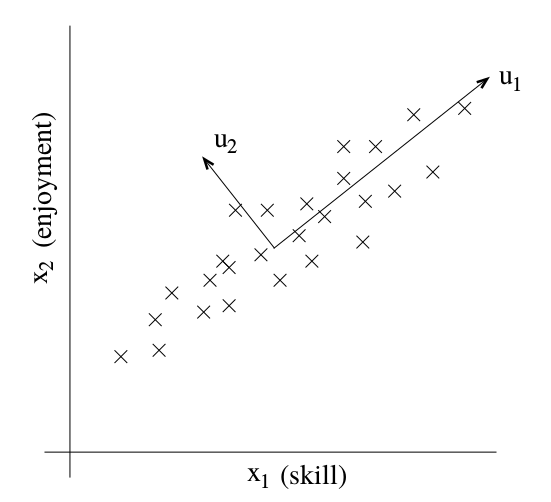
\includegraphics[width=0.4\textwidth]{figures/pca_variance.png}
\caption{Examples.}
\end{figure}

1. Given a set of datasets $X = \{\overrightarrow{x^{(1)}}, \overrightarrow{x^{(2)}}, \cdots, \overrightarrow{x^{(n)}} \}$, we centralize these data and we have
\begin{equation}
\begin{split}
\overrightarrow{\mu} &= \frac{1}{n} \sum_{i=1}^n \overrightarrow{x^{(i)}}, \\
\{\overrightarrow{x^{(1)}}, \overrightarrow{x^{(2)}}, \cdots, \overrightarrow{x^{(n)}} \} &= \{\overrightarrow{x^{(1)}} - \overrightarrow{\mu}, \overrightarrow{x^{(2)}} - \overrightarrow{\mu}, \cdots, \overrightarrow{x^{(n)}}-\overrightarrow{\mu} \}
\end{split}
\end{equation}

2. Find a vector $\vec{u}$ and the projection variance of the data in this direction is the largest. Then, the optimization objective is
\begin{equation}
\begin{split}
\arg \max_{\vec{u}} \frac{1}{n}\sum_{i=1}^m (\overrightarrow{x^{(i)}}^\top \vec{u})^2 &= \frac{1}{n} \sum_{i=1}^n \vec{u}^\top \overrightarrow{x^{(i)}} \overrightarrow{x^{(i)}}^\top \vec{u} \\
&= \vec{u}^\top \left(\frac{1}{n}\sum_{i=1}^m \overrightarrow{x^{(i)}} \overrightarrow{x^{(i)}}^\top \right) \vec{u} \\
&= \vec{u}^\top \left(\frac{1}{n} XX^\top \right) \vec{u} \\
&= \vec{u}^\top \left(\frac{1}{\sqrt{n}} X \frac{1}{\sqrt{n}}X^\top \right)\vec{u} \\
&= \vec{u}^\top \left(Y Y^\top \right)\vec{u}.
\end{split}
\end{equation}

We can know that $Y Y^\top$ in above equation is a positive semi-definite symmetric matrix. Because (1) $Y Y^\top$ is symmetric according to $(YY^\top)^\top = YY^\top$; (2) $Y Y^\top$ ispositive semi-definite according to $\xi^\top Y Y^\top \xi = (Y Y^\top \xi)^\top(Y Y^\top \xi) = ||Y Y^\top \xi||_2^2 \geq 0.$ Therefore, $\vec{u}^\top Y Y^\top \vec{u}$ is a positive semi-definite quadratic form, which has the maximum value.

Because there are another constraint $||\vec{u}|| = \vec{u}^\top \vec{u} = 1$, we usually can solve above problem by Lagrange multiplier method.
\begin{equation}
\begin{split}
f(\vec{u}) &= \vec{u}^\top Y Y^\top \vec{u} + \lambda (1 - \vec{u}^\top \vec{u}), \\
\frac{\partial f(\vec{u})}{\partial \vec{u}} &= 2 (Y Y^\top \vec{u}) - 2 \lambda \vec{u} = 0 \Rightarrow Y Y^\top \vec{u} = \lambda \vec{u}.
\end{split}
\end{equation}
Obviously, $\vec{u}$ is the eigenvector corresponding to the eigenvalue $\lambda$ of $Y Y^\top$. And all the eigenvalues (eigenvectors) of $Y Y^\top$ satisfy the above formula. Then, we have
\begin{equation}
\begin{split}
\vec{u}^\top \left(Y Y^\top \right)\vec{u} = \lambda \vec{u}^\top \vec{u} = \lambda.
\end{split}
\end{equation}
So, we can see that the eigenvalue $\lambda$ is the value of objective funtion. If the maximum eigenvalue is taken, then the value of objective function is taken to the maximum. Therefore, we can decompose the eigenvalues of $Y Y^\top$ to obtain the largest $k$ eigenvalues, and then obtain new samples of $k$-dimensional features by $\overrightarrow{x^{(i)}}^\top \vec{u}$.

\section{Hidden Markov model (HMM)}
\begin{figure}[h]
\label{fig:hmm}
\centering
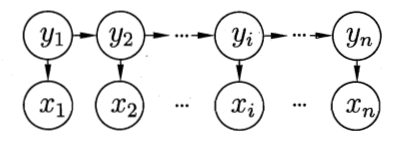
\includegraphics[width=0.4\textwidth]{figures/hmm.png}
\caption{HMM}
\end{figure}

\subsection{Definition}
As shown in Fig.~\ref{fig:hmm}, $y_i$ is the \uline{state sequence} that is produced by the hidden Markov chain, while $x_i$ is the \uline{observation sequence}, which is prodeced by each state $y_i$.

Suppose that the set of state is $Q$ and the set of observation is $V$. Moreover, we give the state sequence $I$ with length $T$ and the observation sequence $O$ with length $T$.
\begin{equation}
\begin{split}
& Q = \{q_1, q_2, \cdots, q_N\}, V = \{v_1, v_2, \cdots, v_M\}, \\
& I = \{i_1, i_2, \cdots, i_T\}, O = \{o_1, o_2, \cdots, o_T\}.
\end{split}
\end{equation}

Next, we define the state transition probability matrix as $A$:
\begin{equation}
A = \left[ a_{ij} \right]_{N \times N}, a_{ij} = P(i_{t+1} = q_j|i_t = q_i).
\end{equation}
Also, we define the observation probability matrix as $B$:
\begin{equation}
B = \left[ b_{ij} \right]_{N \times M}, b_{ij} = P(o_{t} = q_j|i_t = q_i).
\end{equation}
In addition, we define the intial state probability vector $\vec{\pi}$:
\begin{equation}
\vec{\pi} = (\pi_i), \pi_i = P(i_1 = q_i).
\end{equation}

\uline{The two main hypotheses of Hidden Markov model includes: (1) homogeneous Markov hypothesis, (2) observation independence hypothesis}.

\subsection{Three basic problems}
1. Probability calculation problem: given the model $\lambda = \{A, B, \vec{\pi}\}$ and observation sequence $O = \{o_1, o_2, \cdots, o_T\}$, calculate the probability of $P(O|\lambda)$; 
\note[inline]{forward-backward algorithm}

2. Learning problem: given the observation sequence $O = \{o_1, o_2, \cdots, o_T\}$, estimate the model parameters $\lambda = \{A, B, \vec{\pi}\}$;
\note[inline]{Baum-Welch algorithm}

3. Predicting problem (decoding problem): given the model $\lambda = \{A, B, \vec{\pi}\}$ and observation sequence $O = \{o_1, o_2, \cdots, o_T\}$ \, estimate the state sequence. 
\note[inline]{Viterbi algorithm}

\section{Conditional random field (CRF)}
\subsection{Probabilistic undirected graphical model, or Markov random field}
\subsection{Conditional random field}
Let $X$ and $Y$ be random variables, and $P(Y|X)$ be the conditional probability distribution of $Y$ given $X$. If the random variable $Y$ forms a Markov random field represented by and undirected graph $G=(V, E)$, \ie
\begin{equation}
P(Y_v | X, Y_w, w \neq v) = P(Y_v | X, Y_w, w \sim v),
\end{equation}
where $w \neq v$ and $w \sim v$ represents no connection and connection respectively, the conditional probability distribution $P(Y|X)$ is called a conditional random field.

Let $P(Y|X)$ be a linear chain chonditional random field, the conditional probability of random variable $Y = y$ given randome variable $X = x$:
\begin{equation}
\begin{split}
& P(y|x) = \frac{1}{Z(x)} \exp \left( \sum_k \lambda_k \sum_i t_k(y_{i-1}, y_i, x, i) + \sum_l \mu_l \sum_i s_l(y_i, x, i) \right), \\
& Z(x) = \sum_y \exp\left( \sum_k \lambda_k \sum_i t_k(y_{i-1}, y_i, x, i) + \sum_l \mu_l \sum_i s_l(y_i, x, i) \right).
\end{split}
\end{equation}
where $t_k$ and $s_l$ are feature function, and the former is transition feature and latter is state feature. $\lambda_k$ and $u_l$ are weights.

Above formula has a simpler form:
\begin{equation}
\begin{split}
& P(y|x) = \frac{1}{Z(x)} \exp \sum_{k} w_k f_k(y, x), \\
& Z(x) = \sum_y \exp \sum_{k} w_k f_k(y, x).
\end{split}
\end{equation}

\todo[inline]{CRF algorithm}

\section{Generative model and discriminative model}

1. Generative model: naive bayes; hidden Markov model (HMM);

2. Discriminative model: perceptron; Conditional random field (CRF)

\improvement[inline]{Todo: Random forest}

\chapter{Deep Network}
\section{How does backpropagation work?}
\begin{figure}[h]
\centering
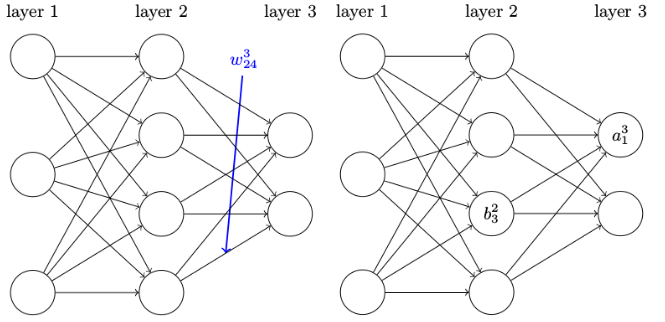
\includegraphics[width=0.5\textwidth]{figures/neural_network.png}
\caption{Neural network.}
\end{figure}
First, symbol definition is carried out. We use $w^l_{jk}$ to denote the weight for the connection from the $k$th neuron in the $(l - 1)$th layer to the $j$th neuron in the $l$th layer. Moreover, we use $b^l_j$ for the bias of $j$th neuron in $l$th layer and we use $a^l_j$ for the activation of the $j$th neuron in $l$th layer. We also use $z^l_j$ as the \uline{weighted input}  of $j$th neuron in $l$th layer. Then
\begin{equation}
\begin{split}
z^l_j & = \sum_k w^l_{jk} a^{l - 1} _ k + b^l_j, \\
a^l_j & = \sigma(\sum_k w^l_{jk} a^{l - 1} _ k + b^l_j) \\
	  & = \sigma(z^l_j).
\end{split}
\label{eq:neural_network}
\end{equation}
where $\sigma$ is the activation function, such as Sigmoid function. Then, Eq.~\ref{eq:neural_network} can be expresented in a vector form. In detail, we use $\vec{a^l}$ for the activation vector in $l$th layer. $\vec{z^l}$ is the same. Moreover, we use $\bm{w^l}$ for the \uline{weight matrix} and $\vec{b^l}$ for the bias vector in $l$th layer. Then, 
\begin{equation}
\begin{split}
\overrightarrow{z^l} & = \bm{w^l}\overrightarrow{a^{l - 1}} + \overrightarrow{b^l}, \\
\overrightarrow{a^l} & = \sigma(\bm{w^l}\overrightarrow{a^{l - 1}} + \overrightarrow{b^l}) \\
		  & = \sigma(\overrightarrow{z^l}).
\end{split}
\end{equation}

The understanding of backpropagation is about how to chang the weights and biases in a network to change the cost function. Utimately, this means computing the partial derivatives $\frac{\partial \mathcal{L}}{\partial w^l_{jk}} $ and $\frac{\partial \mathcal{L}}{\partial b^l_j} $. To compute those, we first introduce an intermedia quantity $\delta^l_j$, which we call the \uline{error} of the $j$th neuroon in the $l$th layer. In the actual calculation process, backpropagation will give us a predure to compute $\delta^l_j$, and then will relate $\delta^l_j$ to $\frac{\partial \mathcal{L}}{\partial w^l_{jk}} $ and $\frac{\partial \mathcal{L}}{\partial b^l_j} $.

We define the error of the $j$th neuroon in the $l$th layer by
\begin{equation}
\delta^l_j = \frac{\partial \mathcal{L}}{\partial z^l_j}.
\end{equation}
Then, we can get \uline{the error of the output layer} $\delta^L$, and the components of $\delta^L$ are given by
\begin{equation}\label{eq:backpropagation_1}
\begin{split}
\delta^L_j & = \frac{\partial \mathcal{L}}{\partial z^L_j} 
		   = \frac{\partial \mathcal{L}}{\partial a^L_j}\frac{\partial a^L_j}{\partial z^L_j} \\
		   & = \frac{\partial \mathcal{L}}{\partial a^L_j} \sigma'(z^L_j).
\end{split}
\tag{BP1}
\end{equation}
Moreover, we can give the matrix-based form of Eq.~\ref{eq:backpropagation_1} by
\begin{equation}
\overrightarrow{\delta^L} = \nabla_{\overrightarrow{a^L}}\mathcal{L} \otimes \sigma'(\overrightarrow{z^L}).
\end{equation}

Then, we can obtain \uline{the error $\delta^l$ in terms of the error in the next layer $\delta^{l+1}$}. In particular, 
\begin{equation}\label{eq:backpropagation_2}
\begin{split}
\delta^l_j & = \frac{\partial \mathcal{L}}{\partial z^l_j} 
		    = \sum_k \frac{\partial \mathcal{L}}{\partial z^{l+1}_k} \frac{\partial z^{l+1}_k}{\partial z^l_j}
		    = \sum_k \delta^{l+1}_k \frac{\partial z^{l+1}_k}{\partial z^l_j} \\
		   & = \sum_k \delta^{l+1}_k \frac{\partial \sum_j w^{l+1}_{kj} \sigma(z^l_j) + b^l_k}{\partial z^l_j} \\
		   & = \sum_k \delta^{l+1}_k w^{l+1}_{kj} \sigma'(z^l_j)
\end{split}
\tag{BP2}
\end{equation}
Moreover, we can give the matrix-based form of Eq.~\ref{eq:backpropagation_2} by
\begin{equation}
\begin{split}
\overrightarrow{\delta^l} = ((\overrightarrow{w^{l+1}})^\mathrm{T}\delta^{l+1}) \otimes \sigma'(\overrightarrow{z^l}).
\end{split}
\end{equation}

Next, we can obtain \uline{the rate of change of the cost with respect to any weight in the network}. In particlular, 
\begin{equation}\label{eq:backpropagation_3}
\begin{split}
\frac{\partial \mathcal{L}}{\partial w^l_{jk}} & = \frac{\partial \mathcal{L}}{\partial z^l_j} \frac{\partial z^l_j}{\partial w^l_{jk}}
	= \frac{\partial \mathcal{L}}{\partial z^l_j} \frac{\partial \sum_k w^l_{jk} a^{l-1}_k + b^l_j}{\partial w^l_{jk}} \\
	& = \frac{\partial \mathcal{L}}{\partial z^l_j} a^{l - 1}_k \\
	& = \delta^l_j a^{l - 1}_k.
\end{split}
\tag{BP3}
\end{equation}
Moreover, we can give the matrix-based form of Eq.~\ref{eq:backpropagation_3} by
\begin{equation}
\frac{\partial \mathcal{L}}{\partial \bm{w^l}} = \overrightarrow{\delta^l} (\overrightarrow{a^{l-1}})^\mathrm{T}.
\end{equation}

We can obtain \uline{the rate of change of the cost with respect to any bias in the network}. In particlular, 
\begin{equation}\label{eq:backpropagation_4}
\begin{split}
\frac{\partial \mathcal{L}}{\partial b^l_j} & = \frac{\partial \mathcal{L}}{\partial z^l_j} \frac{\partial z^l_j}{\partial b^l_j}
	= \frac{\partial \mathcal{L}}{\partial z^l_j} \frac{\partial \sum_k w^l_{jk} a^{l-1}_k + b^l_j}{\partial b^l_j} \\
	& = \frac{\partial \mathcal{L}}{\partial z^l_j} \\
	& = \delta^l_j.
\end{split}
\tag{BP4}
\end{equation}
Moreover, we can give the matrix-based form of Eq.~\ref{eq:backpropagation_4} by
\begin{equation}
\frac{\partial \mathcal{L}}{\partial \overrightarrow{b^l}} = \overrightarrow{\delta^l}.
\end{equation}

\section{Backpropagation of Convolutional Neural Network}
\subsection{Backpropagation of Fully Connectional Layer}
The backprogapation equations of element form are as follows: 
\begin{equation}
\left\{
\begin{split}
& \delta^L_j = \frac{\partial \mathcal{L}}{\partial a^L_j} \sigma'(z^L_j), \\
& \delta^l_j = \sum_k \delta^{l+1}_k w^{l+1}_{kj} \sigma'(z^l_j), \\
& \frac{\partial \mathcal{L}}{\partial w^l_{jk}} = \delta^l_j a^{l - 1}_k, \\
& \frac{\partial \mathcal{L}}{\partial b^l_{j}} = \delta^l_j. \\
\end{split}
\right.
\tag{FC-BP}
\end{equation}

The backprogapation equations of matrix-based form are as follows:
\begin{equation}
\left\{
\begin{split}
& \overrightarrow{\delta^L} = \nabla_{\overrightarrow{a^L}}\mathcal{L} \otimes \sigma'(\overrightarrow{z^L}), 
\\
& \overrightarrow{\delta^l} = ((\overrightarrow{w^{l+1}})^\mathrm{T} \overrightarrow{\delta^{l+1}}) \otimes \sigma'(\overrightarrow{z^l}), 
\\
& \frac{\partial \mathcal{L}}{\partial \bm{w^l}} = \overrightarrow{\delta^l} (\overrightarrow{a^{l-1}})^\mathrm{T}, 
\\
& \frac{\partial \mathcal{L}}{\partial \overrightarrow{b^l}} = \overrightarrow{\delta^l}. \\
\end{split}
\right.
\end{equation}

\subsection{Backpropagation of Convolutional Layer}
We use $w^l_{pq}$ to denote the weight of the element in the $p$th row and $q$th column of the convolutional kernel in $l$th layer. Moreover, $a^l_{ij}$ and $z^l_{ij}$ as the activation and weighted input in $i$th row and $j$th column in $l$th layer, respectively. Then, 
\begin{equation}
\label{eq:convolutional_layer}
\begin{split}
& z^l_{ij} = \sum^r_{p=1} \sum^c_{q=1}  a^{l-1}_{i+p-1, j+q-1} w^l_{pq} + b^l, \\
& a^l_{ij} = \sigma(z^l_{ij}),
\end{split}
\end{equation}
where $\sigma$ is the activation function, such as Sigmoid function. The matrix-based form of Eq.~\ref{eq:convolutional_layer} can be given by
\begin{equation}
\begin{split}
& \bm{z^l} = \bm{a^{l-1}} * \bm{w^l} + \bm{b^l}, \\
& \bm{a^l} = \sigma(\bm{z^l}).
\end{split}
\end{equation}

Similar to fully connectional layer, we define $\delta^l_{ij}$ as the error in element at $i$th row and $j$th column in $l$ layer. In detail, 
\begin{equation}
\begin{split}
\delta^l_{ij} = \frac{\partial \mathcal{L}}{\partial z^l_{ij}}.
\end{split}
\end{equation}
In this equation, $\delta^L$ can be obtain by the same manner as Eq.~\ref{eq:backpropagation_1}. Then, we can obtain the error $\delta^l$ in the terms of the error in the next layer $\delta^{l+1}$. In particular, 
\begin{equation}
\begin{split}
\delta^l_{ij} &= \frac{\partial \mathcal{L}}{\partial z^l_{ij}} 
= \sum_m \sum_n \frac{\partial \mathcal{L}}{\partial z^{l+1}_{mn}} \frac{\partial z^{l+1}_{mn}}{\partial z^l_{ij}} 
\\
&= \sum_m \sum_n \delta^{i+1}_{mn} \frac{\partial z^{l+1}_{mn}}{\partial z^l_{ij}} 
\\
&= \sum_m \sum_n \delta^{i+1}_{mn} \frac{\partial \sum^r_{p=1} \sum^c_{q=1} \sigma(z^{l}_{m+p-1,n+q-1}) w^{l+1}_{pq} + b^{l+1}}{\partial z^l_{ij}} 
\\
&= \sum_m \sum_n \delta^{l+1}_{mn} w^{l+1}_{i+1-m,j+1-n} \sigma'(z^l_{ij}).
\end{split}
\label{eq:convolutional_layer_backpropagation_2}
\tag{CONV-BP2}
\end{equation}
In this case, a example can be found:   
\begin{equation}
\begin{split}
\delta^l_{1,1} = & \delta^{l+1}_{-1,-1} w^{l+1}_{3,3} + \delta^{l+1}_{-1,0} w^{l+1}_{3,2} + \delta^{l+1}_{-1,1} w^{l+1}_{3,1} +  \\
&\delta^{l+1}_{0,-1} w^{l+1}_{2,3} + \delta^{l+1}_{0,0} w^{l+1}_{2,2} + \delta^{l+1}_{0,1} w^{l+1}_{2,1} + \\
&\delta^{l+1}_{1,-1} w^{l+1}_{1,3} + \delta^{l+1}_{1,0} w^{l+1}_{1,2} + \delta^{l+1}_{1,1} w^{l+1}_{1,1},
\end{split}
\end{equation}
which can be represented as convolutional operations like:
\begin{equation}
\left[
\begin{array}{cccccc}
0 & 0 & 0 & 0 & 0 & 0 \\
0 & 0 & 0 & 0 & 0 & 0 \\
0 & 0 & \delta^{l+1}_{1,1} & \delta^{l+1}_{1,2} & 0 & 0 \\
0 & 0 & \delta^{l+1}_{2,1} & \delta^{l+1}_{2,2} & 0 & 0 \\
0 & 0 & 0 & 0 & 0 & 0 \\
0 & 0 & 0 & 0 & 0 & 0 \\
\end{array}
\right]*
\left[
\begin{array}{ccc}
w^{l+1}_{3,3} & w^{l+1}_{3,2} & w^{l+1}_{3,1} \\
w^{l+1}_{2,3} & w^{l+1}_{2,2} & w^{l+1}_{2,1} \\
w^{l+1}_{1,3} & w^{l+1}_{1,2} & w^{l+1}_{1,1} \\
\end{array}
\right].
\end{equation}
Therefore, Eq.~\ref{eq:convolutional_layer_backpropagation_2} can be deduced into matrix-based form, $i.e.$,
\begin{equation}
\bm{\delta^l} = \bm{\delta^{l+1}}*\mathrm{rot180}(\bm{w}) \otimes \sigma'(\bm{z^l}).
\end{equation}

Next, we can calculate the change rate of the cost with respect to any weight in the network. In particular, 
\begin{equation}
\begin{split}
\frac{\partial \mathcal{L}}{\partial w^l_{pq}} &= \sum_i \sum_j \frac{\partial \mathcal{L}}{\partial z^l_{ij}} \frac{\partial z^l_{ij}}{\partial w^l_{pq}} 
\\
&= \sum_i \sum_j \frac{\partial \mathcal{L}}{\partial z^l_{ij}} \frac{\partial \sum^r_{p=1} \sum^c_{q=1}  a^{l-1}_{i+p-1, j+q-1} w^l_{pq} + b^l}{\partial w^l_{pq}} 
\\
&= \sum_i \sum_j \delta^l_{ij} a^{l-1}_{i+p-1,j+q-1}. \\
\end{split} 
\tag{CONV-BP3}
\end{equation}
As for bias, we have 
\begin{equation}
\begin{split}
\frac{\partial \mathcal{L}}{\partial b^l} &= \sum_i \sum_j \frac{\partial \mathcal{L}}{\partial z^l_{ij}} \frac{\partial z^l_{ij}}{\partial b^l} 
\\
&= \sum_i \sum_j \frac{\partial \mathcal{L}}{\partial z^l_{ij}} \frac{\partial \sum^r_{p=1} \sum^c_{q=1}  a^{l-1}_{i+p-1, j+q-1} w^l_{pq} + b^l}{\partial b^l} 
\\
&= \sum_i \sum_j \delta^l_{ij}. \\
\end{split} 
\tag{CONV-BP4}
\end{equation}
In summary, the backpropagation equations of element form for convolutional layer as follows:
\begin{equation}
\left\{
\begin{split}
& \delta^l_{ij} = \sum_m \sum_n \delta^{l+1}_{mn} w^{l+1}_{i+1-m,j+1-n} \sigma'(z^l_{ij}), \\
& \frac{\partial \mathcal{L}}{\partial w^l_{pq}} = \sum_i \sum_j \delta^l_{ij} a^{l-1}_{i+p-1,j+q-1}, \\
& \frac{\partial \mathcal{L}}{\partial b^l} = \sum_i \sum_j \delta^l_{ij}. \\
\end{split}
\right.
\tag{CONV-BP}
\end{equation}
Moreover, the corresponding matrix form is as follows:
\begin{equation}
\left\{
\begin{split}
& \bm{\delta^l} = \bm{\delta^{l+1}}*\mathrm{rot180}(\bm{w}) \otimes \sigma'(\bm{z^l}), \\
& \frac{\partial \mathcal{L}}{\partial \bm{w^l}} = \bm{a^{l-1}}*\bm{\delta^l}, \\
& \frac{\partial \mathcal{L}}{\partial \bm{b^l}} = \sum_{i,j}\bm{b^l}.
\end{split}
\right.
\end{equation}

\section{Why does batch normalization work?}
\subsection{Dataset shift and covariate shift}
There exists a inherent hypothesis in supervised learning: \uline{The training data in source domain and testing data in target domain are independent and identically drawn from the same distribution}. 

Usually, the distrbutions of training data and testing data are not exactly the same, especiallt when the training data is insufficient. This phenomenon is named as ``\uline{dataset shift}''. 

In analysis of covariance (ANOVA), convate is any continuous variable that is usually not controlled during data collection. (referring to \url{https://support.minitab.com/en-us/minitab/18/help-and-how-to/modeling-statistics/anova/supporting-topics/anova-models/understanding-covariates/}). 

For the input variable $x$ (also named as explanatory variable or covariate in scene of batch normalizatio), $y$ is the corresponding label, which is regarded as response variable. If the conditional probabilities of training data and testing data are the same but the marinal probabilities are different, $i.e.$
\begin{equation}\label{eq:covariate_shift}
\begin{split}
P_{tr}(y|x) & = P_{te}(y|x) \\
P_{tr}(x) & \ne p_{te}(y)
\end{split},
\end{equation}
we call this phenomenon as ``\uline{covariate shift}''. Covariate shift is a special kind of dataset shift. 

Moreover, we can deduce the Eq.~\ref{eq:covariate_shift} as follows:
\begin{equation}
\begin{split}
P_{tr}(x, y) = P_{tr}(y|x)P_{tr}(x) \\
P_{te}(x, y) = P_{te}(y|x)P_{te}(x)
\end{split},
\end{equation}
and we know the joint probabilities of traning data and testing data are different, $i. e.$, 
\begin{equation}\label{eq:covariate_shift_2}
P_{tr}(x, y) \ne P_{te}(x, y).
\end{equation}.
From Eq.~\ref{eq:covariate_shift_2}, this scene violates the independence hypothesis of supervised learning, so the prediction is inaccurate.

\unsure[inline]{A more precise definition of \textbf{covariate} can't be found.}

\subsection{Internal covariate shift}
\uline{Internal covariate shift} is defined as the change in the distribution of network activations due to the change in network parameters during training. 


\begin{figure}[h]
\centering
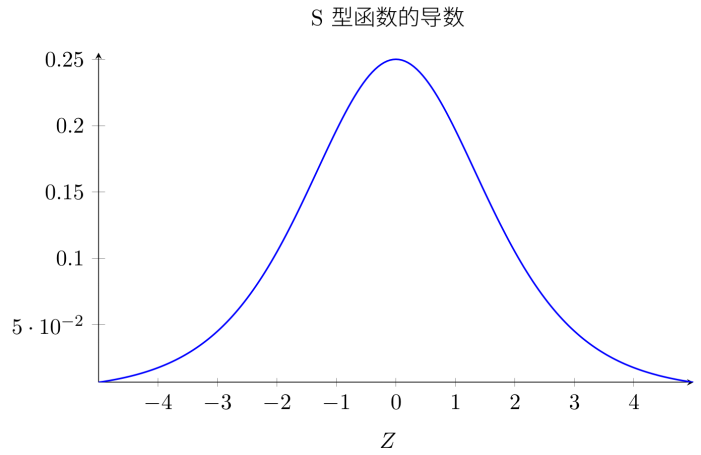
\includegraphics[width=0.8\textwidth]{figures/sigmoid.png}
\caption{Derivative of sigmoid function.}
\end{figure}


\textbf{Consequences of internal covariate shift: }(1) Intuitively, the layers need to continuously adapt to the new distribution, which lead to a decrease in training speed. (2) Objectively, the changes of $W$ and $b$ during training will likely move many dimensions of $x$ into the saturated regime of the nonlinearity ($e.g.$ sigmoid and tanh) and slow down the convergence. The saturation problem is usually addressed by using ReLU, careful initialization and small learning rates. Moreover, if the distribution of nonlinearity inputs remains more stable at the sensitive regions in nonlinearity as the network trains, the optimizer would be less likely to get stuck in the staturated regime, and the training would accelerate.

\improvement[inline]{PCA whitening and ZCA Whitening.}

\subsection{Batch normalization}
\label{sect:batch-normalization}
\textbf{Problem: } because whitening is expensive and maybe change the representation ability of a network by discarding the absolute scale of activations, batch nomalization emerges.

There are two treatments for batchnorm to address above two problems. (1) The first is instead of whitening the features in layer inputs and outputs jountly, batchnorm normalizes each scalar feature independently, by making it have the mean of 0 and the variance of 1. For a layer with $d$-dimensional input $x=[x^{(1)}, x^{(2)}, \cdots, x^{(k)}]$,  each dimension is normalized as follows 
\begin{equation}
\hat{x}^{(k)} = \frac{x^{(k)} - E[x^{(k)}]}{\sqrt{Var(x^{(k)})}}.
\end{equation}
(2)Simply normalizeing each input of a layer may reduce what the layer can represent. For example, nomalizing the inputs of a sigmoid would constrain them to the linear regime of the nonlinearity.
\begin{figure}[h]
\centering
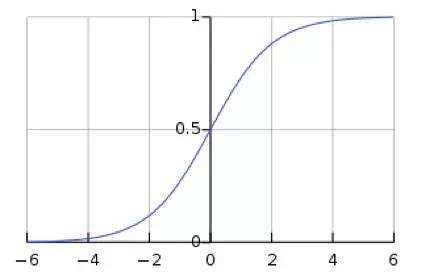
\includegraphics[width=0.5\textwidth]{figures/sigmoid_batchnorm.png}
\caption{Sigmoid function.}
\end{figure}
In this way, batchnorm turns the multi-layer nonlinear neural network into a multi-layer linear neural network, which is equivalent to the representation ability of a single layer linear network. The reduces the representation ability of the network. So, introduce $\gamma ^ {(k)}, \beta^{(k)}$ to scale and shift the normalized value:
\begin{equation}
y^{(k)} = \gamma ^ {(k)} \hat{x} ^ {(k)} + \beta ^ {(k)},
\end{equation}
which guarantee the representation ability of the network.
\improvement[inline]{Why is multi-layr linear network equivalent to the represetation ability of a single layer linear network.}

In addition, use mini-batch in stochatic gradient training, each mini-batch produces estimates of the man and variance of each activation. And obtain the forward algorithm of batch normalization as follows: \\

\begin{algorithm}
	\renewcommand{\algorithmicrequire}{\textbf{Input:}}
	\renewcommand{\algorithmicensure}{\textbf{Output:}}
	\caption{Forward algorithm of batch normalization.}
	\begin{algorithmic}[1]
		\REQUIRE values of $x$ over a mini-batch: $\mathcal{B}=\{x_1, x_2, \cdots, x_m\}$, parameters to be learned: $\gamma, \beta$
		\ENSURE$y_i = BN_{\gamma, \beta}(x_i)$
		\begin{equation}
		\begin{split}
		& \mu_\mathcal{B} \gets \frac{1}{m} \sum_{i=1}^m x_i \\
		& \sigma^2_\mathcal{B} \gets \frac{1}{m} \sum_{i=1}^m (x_i - \mu_\mathcal{B})^2 \\
		& \hat{x}_i \gets \frac{x_i - \mu_\mathcal{B}}{\sqrt{\sigma^2_\mathcal{B} + \epsilon}} \\
		& y_i \gets \gamma\hat{x}_i + \beta = BN_{\gamma, \beta}(x_i)
		\end{split}
		\notag
		\end{equation}
	\end{algorithmic}  
\end{algorithm}
In this manner, we know 
\begin{equation}
\begin{split}
E[\hat{x}] &= E[\frac{x_i - \mu_\mathcal{B}}{\sqrt{\sigma^2_\mathcal{B} + \epsilon}}] \\
		&= \frac{1}{\sqrt{\sigma^2_\mathcal{B} + \epsilon}} (E[x_i] - E[\mu_\mathcal{B}]) \\
		&= 0 \\
Var[\hat{x}] &= E[\hat{x}^2] - (E[\hat{x}])^2 \\
			&= E[(\frac{x_i - \mu_\mathcal{B}}{\sqrt{\sigma^2_\mathcal{B} + \epsilon}})^2] + 0 \\
			& = \frac{1}{\sigma^2_\mathcal{B} + \epsilon} E[(x_i - \mu_\mathcal{B})^2] \\
			& = \frac{1}{\sigma^2_\mathcal{B} + \epsilon} \sigma^2_\mathcal{B} \\
			& \approx 1
\end{split}.
\end{equation}
The distribution of values of any $\hat{x}$ has the expected value of 0 and the invariance of 1, as long as the elements of each mini-batch are sampled from the same distribution, and if we neglect $\epsilon$. This distribution can be seen as an approximate standard normal distribution $N(0, 1)$.

We compute the gradients with respect to the parameters of the BN thansform of loss $\mathcal{L}$ for backpropagation. The chain rule is used as follows:
\begin{equation}
\begin{split}
& \frac{\partial \mathcal{L}}{\partial \gamma} = \sum_i \frac{\partial \mathcal{L}}{\partial y_i}  \frac{\partial y_i}{\partial \gamma} = \sum_i \frac{\partial \mathcal{L}}{\partial y_i} \hat{x}_i, \\
& \frac{\partial \mathcal{L}}{\partial \beta} = \sum_i \frac{\partial \mathcal{L}}{\partial y_i}  \frac{\partial y_i}{\partial \beta} = \sum_i \frac{\partial \mathcal{L}}{\partial y_i}. \\
\end{split}
\end{equation}
\note[inline]{There exists $\sum_i$ for $y_i$ because gradient from each $y_i$ will backpropagate for $\gamma$ and the effect of summation is achieved.}
For the process of \textbf{backpropagation}, we also need to compute $\frac{\partial \mathcal{L}}{\partial x_i}$, which is got by:
\begin{equation}
\begin{split}
\frac{\partial \mathcal{L}}{\partial \hat{x}_i} & = \frac{\partial \mathcal{L}}{\partial y_i}  \frac{\partial y_i}{\partial \hat{x}_i} \\
&= \frac{\partial \mathcal{L}}{\partial y_i} \gamma 
\\
\frac{\partial \mathcal{L}}{\partial \sigma^2_\mathcal{B}} &= \sum_i \frac{\partial \mathcal{L}}{\partial \hat{x}_i}  \frac{\partial \hat{x}_i}{\partial \sigma^2_\mathcal{B}} \\
&= \sum_i \frac{\partial \mathcal{L}}{\partial \hat{x}_i} (x_i - \mu_\mathcal{B}) (-\frac{1}{2}) (\sigma^2_\mathcal{B} + \epsilon)^{-\frac{3}{2}} \\
&=-\frac{1}{2} \sum_i \frac{\partial \mathcal{L}}{\partial \hat{x}_i} (x_i - \mu_\mathcal{B}) (\sigma^2_\mathcal{B} + \epsilon)^{-\frac{3}{2}} 
\\
\frac{\partial \mathcal{L}}{\partial \mu_\mathcal{B}} &= \frac{\partial \mathcal{L}}{\partial \hat{x}_i} \frac{\partial \hat{x}_i}{\partial \mu_\mathcal{B}} + \frac{\partial \mathcal{L}}{\partial \sigma^2_\mathcal{B}} \frac{\partial \sigma^2_\mathcal{B}}{\partial \mu_\mathcal{B}} \\
&= \sum_i \frac{\partial \mathcal{L}}{\partial \hat{x}_i}(-1)(\sigma^2_\mathcal{B} + \epsilon)^{-\frac{1}{2}} + \frac{\partial \mathcal{L}}{\partial \sigma^2_\mathcal{B}}\frac{1}{m}\sum_i (-2) (x_i - \mu_\mathcal{B}) \\
&= -\sum_i \frac{\partial \mathcal{L}}{\partial \hat{x}_i}\frac{1}{\sqrt{\sigma^2_\mathcal{B} + \epsilon}} - \frac{\partial \mathcal{L}}{\partial \sigma^2_\mathcal{B}}\frac{2}{m}\sum_i(x_i - \mu_\mathcal{B})
\\
\frac{\partial \mathcal{L}}{\partial x_i} &= \frac{\partial \mathcal{L}}{\partial \hat{x}_i} \frac{\partial \hat{x}_i}{\partial x_i} + \frac{\partial \mathcal{L}}{\partial \sigma^2_\mathcal{B}} \frac{\partial \sigma^2_\mathcal{B}}{\partial x_i}+ \frac{\partial \mathcal{L}}{\partial \mu_\mathcal{B}} \frac{\partial \mu_\mathcal{B}}{\partial x_i} \\
&= \frac{\partial \mathcal{L}}{\partial \hat{x}_i} \frac{1}{\sqrt{\sigma^2_\mathcal{B} + \epsilon}} + \frac{2}{m} \frac{\partial \mathcal{L}}{\partial \sigma^2_\mathcal{B}} (x_i - \mu_\mathcal{B}) + \frac{1}{m} \frac{\partial \mathcal{L}}{\partial \mu_\mathcal{B}}
\\
\end{split}
\end{equation}

For the \textbf{inference} of the network, sometimes we want the output to depend only on the few or one input. At this time, $\mu$ and $\sigma^2$ are computed by each mini-batch $\mu_\mathcal{B}$ and $\sigma^2_\mathcal{B}$ by their unbiased estimations as proved in~\ref{eq:unbiased_estimation_of_sample_mean_and_variance}:
\begin{equation}
\begin{split}
\mu &= E(\mu_\mathcal{B}), \\
\sigma^2 &= \frac{n}{n-1}E(\sigma^2_\mathcal{B}), \\
BN(X) & = \gamma \frac{X - \mu}{\sqrt{\sigma^2 + \epsilon}} + \beta.
\end{split}
\end{equation}

The advantages of batch normalization is as follows: (1) batch normalization ensure the stable distributions of input in each layer, which reduces the learning pressure at the later layer and improves the learning speed; (2) batch normalization makes the model less sensitive to the parameters in the network, which simplifies the parameter adjustment precess, and makes the learning of this network more stable; (3) batch normalization can make the input of activation fall into the unsaturated region through the normalization operation, thus alleviating the problem of gradient vanishing.

\section{Why does residual learning work?}

\begin{figure}[h]
\centering
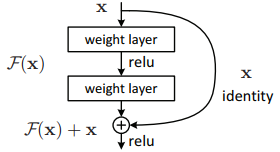
\includegraphics[width=0.4\textwidth]{figures/residual_learning_block.png}
\caption{Residual Learning.}
\end{figure}

In the process of optimization in deep networ
k, the input and output are usually close in the latter layers. In some latter layers, we define the input is $\rm{x}$ and the output is $\mathcal{H(\rm{x})}$. From above experience, we assume $\rm{x}$ and $\mathcal{H(\rm{x})}$ are close. Thus, the function of these layers is mapping from $\rm{x}$ to $\mathcal{H(\rm{x})}$. But usually this process is difficult becuase the relative gap between $\rm{x}$ and $\mathcal{H(\rm{x})}$ is small. Toward this end, we construct the residual as \uline{$\mathcal{F(\rm{x})} = \mathcal{H(\rm{x})} - \rm{x}$} to learning the gap. We can hypothesize that it is easier to optimize the residual mapping than to optimize the original mapping. To the extreme, if the mapping from input to output is indentity, it would be easier to push the residual to zero than to directly fit an identity mapping.

\uline{The real purpose of residual learning is that even if the network deepens, the performance of this network will not degenerate, thus ensuring the leaning of deeper network (even 1000 layers).}

\section{Understanding Deconvolution \& bilinear interpolation}
For the convolutional operation, if we have the input map $I$ and the kernel $K$, we can get the output $O$,
\begin{equation}
\begin{split}
I = \left[
	\begin{matrix}
	4 & 5 & 8 & 7 \\
	1 & 8 & 8 & 8 \\
	3 & 6 & 6 & 4 \\
	6 & 5 & 7 & 8 \\
	\end{matrix} 
	\right],
K = \left[
	\begin{matrix}
	1 & 4 & 1 \\
	1 & 4 & 3 \\
	3 & 3 & 1 \\
	\end{matrix}
	\right].
\end{split}
\end{equation}
When computing convolutional operation by computer, convolutional operation is usually written as matrix multiplication. The form is 
\begin{equation}
M(O) = M(W) M(I),
\end{equation}
where $M(O), M(W)$ and $M(I)$ are matrices of output, weight and input. 
Then, we have the next form,
\begin{equation}\label{eq:matrix_form_of_convolution}
\begin{split}
M(W) = \left[
	\begin{matrix}
	1 & 4 & 1 & 0 & 1 & 4 & 3 & 0 & 3 & 3 & 1 & 0 & 0 & 0 & 0 & 0 \\
	0 & 1 & 4 & 1 & 0 & 1 & 4 & 3 & 0 & 3 & 3 & 1 & 0 & 0 & 0 & 0 \\
	0 & 0 & 0 & 0 & 1 & 4 & 1 & 0 & 1 & 4 & 3 & 0 & 3 & 3 & 1 & 0 \\
	0 & 0 & 0 & 0 & 0 & 1 & 4 & 1 & 0 & 1 & 4 & 3 & 0 & 3 & 3 & 1 \\
	\end{matrix}
	\right],
M(I) = \left[
	\begin{matrix}
	4 \\
	5\\
	8\\
	7\\
	1\\
	8\\
	8\\
	8\\
	3\\
	6\\
	6\\
	4\\
	6\\
	5\\
	7\\
	8\\
	\end{matrix}
	\right], 
M(O) = M(W) M(I) = \left[
		\begin{matrix}
		122 \\
		148 \\
		126 \\
		134 \\
		\end{matrix}
		\right]
\end{split}
\end{equation}

\subsection{Why is it called Transposed Convolution?}
We can observe that the size of input matrix is $4 \times 4$ and the one of weight is $3 \times 3$, so that the size of output matrix is $2 \times 2$. If we want the get the input by the output $M(O)$ with the convolutional kernel $M(W)$, we can get the input, 
\begin{equation}
M(I) = M(W)^\top M(O).
\end{equation}
which is not the reverse operation of Eq.~\ref{eq:matrix_form_of_convolution} and only represnets the shape restoration.

In the implement of Transposed Convolution, the matrix of weights is transposed, so that the opearation is called \uline{tranposed convolution}.

There are three implementations of transposed convolution. Suppose that $I = [5 \ 8 \ 11], W = [1 \ 2]$.

(1) above matrix form 
\begin{equation}
\begin{split}
M(W)^\top = \left[
	\begin{matrix}
	1 & 0 & 0 \\
	2 & 1 & 0 \\
	0 & 2 & 1 \\
	0 & 0 & 2 \\
	\end{matrix}
\right],
M(I) = \left[
	\begin{matrix}
	5 \\
	8 \\
	11 \\
	\end{matrix}
\right],
M(O) = M(W)^\top M(I) = \left[
	\begin{matrix}
	5 \\
	18 \\
	27 \\
	22 \\
	\end{matrix}
\right].
\end{split}
\end{equation}

(2) pad input and convolve it with rot180$(W)$. For example, input $I$, weight $O$
\begin{equation}
\begin{split}
O & = I * \text{rot180}(W) \\
	&= [0 \ 5 \ 0 \ 8 \ 0 \ 11] * [2 \ 1] \\
	& = [5 \ 18 \ 27 \ 22] 
\end{split}.
\end{equation}

(3) For example,
\begin{equation}
\begin{split}
	\left[
	\begin{matrix}
	5 & 8 & 11
	\end{matrix}
\right] \O  \left[
	\begin{matrix}
	1 & 2
	\end{matrix}
\right] = \left[
	\begin{matrix}
	5*1 & 5*2 + 8*1 & 8*2 + 11*1 & 11 *2
	\end{matrix}
\right] = \left[
	\begin{matrix}
	5 & 18 & 27 & 22
	\end{matrix}.
\right] 
\end{split}
\end{equation}
\todo[inline]{checkerboard artifacts, gridding issues}
\subsection{Bilinear Interpolation}
\begin{figure}[h]
\centering
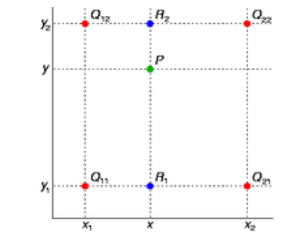
\includegraphics[width=0.4\textwidth]{figures/bilinear.png}
\caption{Bilinear interpolation}
\end{figure}
As shown in Figure, suppose that $Q_{11} = (x_1, y_1), Q_{12} = (x_1, y_2), Q_{21} = (x_2, y_1), Q_{22} = (x_2, y_2)$.
For the point $P = (x, y)$, we can compute the value of $R_{1}$ and $R_2$ firstly.
\begin{equation}
\begin{split}
f(R_1) &= \frac{x_2 - x}{x_2 - x_1} f(Q_{11}) + \frac{x - x_1}{x_2 - x_1} f(Q_{21}), \\
f(R_2) &= \frac{x_2 - x}{x_2 - x_1} f(Q_{12}) + \frac{x - x_1}{x_2 - x_1} f(Q_{22}), \\
f(P) &= \frac{y_2 - y}{y_2 - y_1} f(R_1) + \frac{y - y_2}{y_2 - y_1}f(R_2) \\
	 &= \frac{(x_2 - x)(y_2 - y)}{(x_2 - x_1)(y_2 - y_1)} f(Q_{11}) + \frac{(x - x_1)(y_2 - y)}{(x_2 - x_1)(y_2 - y_1)} f(Q_{21}) \\
	 & + \frac{(x_2 - x)(y - y_2)}{(x_2 - x_1)(y_2 - y_1)} f(Q_{12}) + \frac{(x - x_1)(y - y_2)}{(x_2 - x_1)(y_2 - y_1)} f(Q_{22}) \\   
\end{split}
\end{equation}

In a deep neural network, we usually use bilinear interpolation to upsample a feature map, which is usually implemented by a transposed convolution initialing by bilinear kernel. And the transposed convolution is usually needed to learn. For example, there is a bilinear kernel of size $4 \times 4$.

\begin{equation}
\begin{split}
\left[
\begin{matrix}
	& 0.0625 & 0.1875 & 0.1875 & 0.0625 \\
    & 0.1875 & 0.5625 & 0.5625 & 0.1875 \\
    & 0.1875 & 0.5625 & 0.5625 & 0.1875 \\
    & 0.0625 & 0.1875 & 0.1875 & 0.0625 \\
\end{matrix}
\right].
\end{split}
\end{equation}

There is the code to get the bilinear kernel of size $size$.

\begin{tcolorbox}  
\begin{lstlisting}[language={Python},numbers=left,numberstyle=\tiny,%frame=shadowbox,  
   rulesepcolor=\color{red!20!green!20!blue!20},  
   keywordstyle=\color{blue!70!black},  
   commentstyle=\color{blue!90!},  
   basicstyle=\ttfamily]  
import numpy as np
def upsample_filt(size):  # size = 4 
    """
    Make a 2D bilinear kernel suitable for upsampling of the given (h, w) size.
    """
    factor = (size + 1) // 2  # factor = 2
    if size % 2 == 1:
        center = factor - 1  
    else:
        center = factor - 0.5 # size = 1.5
    og = np.ogrid[:size, :size] 
    return (1 - abs(og[0] - center) / factor) * \
           (1 - abs(og[1] - center) / factor)
upsample_filt(4)
# output
# array([[0.0625, 0.1875, 0.1875, 0.0625],
#       [0.1875, 0.5625, 0.5625, 0.1875],
#       [0.1875, 0.5625, 0.5625, 0.1875],
#       [0.0625, 0.1875, 0.1875, 0.0625]])
upsample_filt(6)
# array([[0.02777778, 0.08333333, 0.13888889, 0.13888889, 0.08333333,
#        0.02777778],
#       [0.08333333, 0.25      , 0.41666667, 0.41666667, 0.25      ,
#        0.08333333],
#       [0.13888889, 0.41666667, 0.69444444, 0.69444444, 0.41666667,
#        0.13888889],
#       [0.13888889, 0.41666667, 0.69444444, 0.69444444, 0.41666667,
#        0.13888889],
#       [0.08333333, 0.25      , 0.41666667, 0.41666667, 0.25      ,
#        0.08333333],
#       [0.02777778, 0.08333333, 0.13888889, 0.13888889, 0.08333333,
#        0.02777778]])
\end{lstlisting} 
\end{tcolorbox}

\section{Activation Function}
Since the preception is equivalent to a NAND gate (which can be regarded as universal gate), the multilayer perception can fit any linear function. However, in general, many problems are not linearly seperable, so it is necessary to introduce nonlinear transformation.

\subsection{Sigmoid}
Simoid is widely used for improving the nondifferentiable jump function. However, in biology, neurons are considered to be sparsely activated, with only 1\%-4\% activated at the same time. Meanwhile, Sigmoid has a amount of computation for derivative calculation and has the problem of gradient vanishing, which leads to the difficult of deep network training. Thus ReLU (2011, Bengio and Xavier) appears.

\subsection{ReLU}
ReLU maybe has the problem of \uline{Dead Neurons}, \ie, some parameters never are activated. The reasons are: (1) bad initialization; (2) the learning rete is too high and the parameters are updated greatly, which makes the network neter this state.

The solutions to above problem include: (1) initializing with Xavier; (2) use adagrad or other methods to adaptively adjust learning rate; (3) use some improvement of ReLU (\eg, leaky ReLU, PReLU and ELU (Exponential ReLU)).

However, the non-linearity of ReLU is weak, which leads to better fitting in deeper network.

\section{Parameter Initialization}
\subsection{Why not initialized with all zeros?}
Take the task of image classification as an example, the sensitivity of neurons in the output layer is $\delta^L_j = \frac{\partial \mathcal{L}}{\partial a^L_j} \sigma'(z^L_j)$ and the gradient of weights in the output layer is $\frac{\partial \mathcal{L}}{\partial w^l_{jk}} = \delta^l_j a^{l - 1}_k$.

For single-layer perceptron (logistic regression), the model can be trained normally. The reason is the different weights $w^l_{jk}$ have different updations. 

But for multi-layer neural network, the training fails. (1) If the activation function of hidden layers is ReLU, all the outputs, graidents and weights in layers are zeros, which means that all the neurons except inputs are dead neurons. Thus the learning fails. (2) If Sigmoid is the used activation function, the neurons can be learned but all the outputs, graidents and weights are same, which means that the learning doesn't work.

\subsection{Why not initialized with Standard Gaussian?}
If there are $n_{in}$ (such as 50) ones in the input layer, the output after first layer is belongs to $\mathcal{N}(0, \sqrt{50})$. After activated, the output saturates. The gradient is about 0 (for Sigmoid) and the learning is slow.

Solution: we usually use the Gaussian Distribution $\mathcal{N}(0, \sqrt{n_{in}})$ to initialize the weights, so that the activation does't fall into the saturation region.

\subsection{xavier}
\textbf{Glorot Condition: }\uline{In order to keep informantion flowing, the invariance of the activation value remains same during forward-propagation and the invariance of the graident with respect to the state value remains same during back-propagation}.

There are some assumptions:
1) the linear activation function is used and the derivative at zero is 1;
2) activation value $x$ and weight $w$ are independent.

Then, we have
\begin{equation}
\begin{split}
a^l_i &= \sum_{k=1}^{n_{in}} w^l_{ik} x^l_{k}, \\
Var(w_{ik} x_k) &= E(w_{ik}^2 x_k^2) - E^2(w_{ik} x_{k}) \\
			&= E(w_{ik}^2) E(x_{k}^2) - E^2(w_{ik})E^2(x_{k}) \\
			&= E^2(w_{ik})Var(x_{k}) + E^2(x_k)Var(w_{ik}) + Var(x_k)Var(w_{ik}). \\ 
\end{split}
\end{equation}
Where $n_{in}$ is the number of input neurons.

If $E(w^l_{ik}) = E(x^l_{k}) = 0$, we have
\begin{equation}\label{eq:xavier_fp}
\begin{split}
Var(a^l_i) &= \sum_{k = 1}^{n_{in}} Var(x^l_{k})Var(w^l_{ik}) \\
		&= {n_{in}} Var(x^l_k) Var(w^l_{ik}) \\
		&= n_{in}Var(x^l) Var(w^l) \\
		&= n_{l - 1} Var(a^{l - 1}) Var(w^l).
\end{split}
\end{equation}

If \uline{the invariance of the activation value remains same during forward-propagation}, we need $Var(a) = Var(x)$ and we have $Var(w) = \frac{1}{n_{in}}$.

If \uline{the invariance of the graident with respect to the state value remains same during back-propagation}, we need $Var(\frac{\partial{\mathcal{L}}}{\partial z^l}) = Var(\frac{\partial{\mathcal{L}}}{\partial z^{l + 1}})$, and we have
\begin{equation}
\begin{split}
Var(\frac{\partial{\mathcal{L}}}{\partial z^l_{i}}) &= 
Var( \sum_{k = 1}^{n_{out}} w^{l+1}_{ik} \frac{\partial{\mathcal{L}}}{\partial z^{l+1}_{k}}  \sigma'(z^l_k)) \\
	&= Var( n_{out} w^{l+1}_{ik} \frac{\partial{\mathcal{L}}}{\partial z^{l+1}_k}) \\
	&= n_{out} Var(w^{l + 1}_{ik}) Var(\frac{\partial{\mathcal{L}}}{\partial z^{l+1}_k}) \\
	&= n_{l+1} Var(w^{l + 1}_{ik}) Var(\frac{\partial{\mathcal{L}}}{\partial z^{l+1}_k}).
\end{split}
\end{equation}
Then, we have $Var(w) = \frac{1}{n_{out}}$. Since $n_{in}$ and $n_{out}$ are usually not equal, the average is taken. Thus we have $Var(w)  = \frac{2}{n_{in} + n_{out}}$.

Under this condition, if $w$ obeys uniform distribution with a mean of 0, then we have $w \sim \mathcal{U}[- \frac{\sqrt{6}}{\sqrt{n_{in} + n_{out}}},  \frac{\sqrt{6}}{\sqrt{n_{in} + n_{out}}}]$.

This is Xavier initialization method. A detailed derivation can be found in the blog \url{https://blog.csdn.net/victoriaw/article/details/73000632}.

\subsection{msra}
In the derivation of xaiver in Eq.~\ref{eq:xavier_fp} and \ref{eq:xavier_bp}, a linear activation function is required. However, ReLU is not a linear function. In general, if ReLU is used, we can't guarancee that \textbf{Glorot Condition} is met (\uline{\ie, the invariance of the activation value remains same during forward-propagation and the invariance of the graident with respect to the state value remains same during back-propagation}).

In order to maintain a stable variance, Kaiming et al. propose a new initialization method and the purpose is to achieve that \uline{the invariance of the state value remains same during forward-propagation and the invariance of the graident with respect to the activation value remains same during back-propagation}.

From this assumption, we have
Then, we have
\begin{equation}
\begin{split}
z^l_i &= \sum_{k=1}^{n_{in}} w^l_{ik} x^l_k, \\
a^l_i &= f(z^l_i), \\
Var(w_{ik} x_k) &= E(w_{ik}^2 x_k^2) - E^2(w_{ik} x_k) \\
			&= E(w_{ik}^2) E(x_k^2) - E^2(w_{ik})E^2(x_k) \\ 
\end{split}
\end{equation}
Where $n_{in}$ is the number of input neurons.

If $E(w_{ik}) = 0$ and $E(x_k) \neq 0$ because the activation function is ReLU,  we have
\begin{equation}\label{eq:msra_fp}
\begin{split}
Var(z^l_i) &= \sum_{k = 1}^{n_{in}} Var(w^l_{ik} x^l_k) \\
		&= {n_{in}} E([w^l_{ik}]^2) E([x^l_i]^2) \\
		&= n_{in} Var(w^l_{ik}) E([x^l_i]^2). \\
E(z^{l - 1}_i) &= E(w^{l - 1}_{ik} x^{l - 1}_k) \\
		&= E(w^{l - 1}_{ik}) E(x^{l - 1}_k) \\
		& = 0 \\
\end{split}
\end{equation}

\begin{equation}
\begin{split}
E([x^l_i]^2) &= E([f(z^{l-1}_i)]^2) \\
		&= \int_{-\infty}^{\infty} p(z^{l-1}_i) [f(z^{l-1}_i)]^2 dz^{l - 1}_i \\
		&= \int_{-\infty}^{0} p(z^{l-1}_i) [f(z^{l-1}_i)]^2 dz^{l - 1}_i + \int_{0}^{\infty} p(z^{l-1}_i) [f(z^{l-1}_i)]^2 dz^{l - 1}_i \\ 
		&= 0 + \int_{0}^{\infty} p(z^{l-1}_i) [z^{l-1}_i]^2 dz^{l - 1}_i \\
		&= \frac{1}{2} \int_{0}^{\infty} p(z^{l-1}_i) [z^{l-1}_i]^2 dz^{l - 1}_i \\
		&= \frac{1}{2} E([z^{l - 1}_i]^2) \\
		&= \frac{1}{2} Var(z^{l - 1}_i) \\
\end{split}
\end{equation}

\begin{equation}
\begin{split}
Var(z^l_i) &= n_{in} Var(w^l_{ik}) E([x^l_i]^2) \\
			&= \frac{1}{2} n_{in} Var(w^l_{ik})  Var(z^{l - 1}_i) \\
\end{split}
\end{equation}

If \uline{the invariance of the state value remains same during forward-propagation}, we need $Var(z^l) = Var(z^{l - 1})$ and we have $Var(w)  = \frac{2}{n_{in}}$.

If \uline{the invariance of the graident with respect to the activation value remains same during back-propagation}, we need $Var(\frac{\partial{\mathcal{L}}}{\partial a^{l}}) = Var(\frac{\partial{\mathcal{L}}}{\partial a^{l + 1}})$, and we have

\begin{equation} \label{eq:activation_bp}
\begin{split}
 \frac{\partial{\mathcal{L}}}{\partial a^l_i} &= \sum_{k=1}^{n_{l+1}} w^{l+1}_{ik} \frac{\partial \mathcal{L}}{\partial a^{l+1}_k}
\end{split} 
\end{equation}

\begin{equation}
\begin{split}
	Var(\frac{\partial{\mathcal{L}}}{\partial a^l_i}) &= n_{l+1} Var(w^{l+1}_{ik} \frac{\partial  \mathcal{L}}{\partial  a^{l+1}_k}) \\
	&= n_{l+1} E([w^{l+1}_{ik}]^2) E([\frac{\partial  \mathcal{L}}{\partial  a^{l+1}_k})]^2) \\
	&= n_{l+1} Var(w^{l+1}_{ik}) E([\frac{\partial  \mathcal{L}}{\partial  a^{l+1}_k}]^2 [\frac{\partial a^{l+1}_k}{\partial  z^{l+1}_k}]^2) \\
	&= n_{l+1} Var(w^{l+1}_{ik}) E([\frac{\partial  \mathcal{L}}{\partial  a^{l+1}_k}]^2) E([f'(z^{l+1}_k)]^2) \\
\end{split} 
\end{equation}

We can know that $E([f'(z^{l+1}_k)]^2) = \frac{1}{2}$. Moreover, from Eq.~\ref{eq:activation_bp}, we can know that $E(\frac{\partial \mathcal{L}}{\partial a^{l+1}_i}) = 0$. Thus we have
\begin{equation}
\begin{split}
	Var(\frac{\partial{\mathcal{L}}}{\partial a^l_i}) &= \frac{1}{2} n_{l+1} Var(w^{l+1}_{ik}) Var(\frac{\partial  \mathcal{L}}{\partial  a^{l+1}_k}). \\
\end{split} 
\end{equation}
And we have that $Var(w^{l+1}_{ik}) = \frac{2}{n_{l+1}}$, \ie $Var(w^{l}_{ik}) = \frac{2}{n_{l}}$.

Under this condition, if $w$ obeys gaussian distribution with a mean of 0, then we have $w \sim \mathcal{N}[0, \frac{2}{n_{in}}]$.

This is Msra initialization method. A detailed derivation can be found in the blog \url{https://blog.csdn.net/VictoriaW/article/details/73166752} and \url{https://www.cnblogs.com/wangguchangqing/p/11013698.html}. \note[inline]{We can know that Xavier and Msra can both belong to uniform distribution or gaussian distribution.}

\chapter{Contents specifically referenced}
\noindent $\bullet$ Sect.~\ref{sect:perceptron}: the chapter of (2)Perceptron in \cite{hangli2012}; \\
$\bullet$ Sect.~\ref{sect:batch-normalization}: BatchNorm from~\cite{ioffe2015batch};

{\small
\bibliographystyle{plain}
\bibliography{RefNote}
}

\end{document}
